\chapter{State of the art} \label{sec:stateofArt}

Text-to-image is an emerging field of deep learning where models can generate lifelike and highly detailed images from textual descriptions. The development of these models is a challenging task that requires the close integration of both computer vision and NLP approaches. The latest advancements in text-to-image models have led to the capability of producing high-quality images with rich semantic content that can now be used for tons of applications including video games and virtual reality, e-commerce, or education among others. Even though recent advancements have allowed the use for commercial applications, generative models remain a challenging and tough problem. This section aims to analyse the current state-of-the-art of text-to-image models.

\section{Historical review of text-to-image models} \label{Hreview}

Text-to-image models have been present among researchers for a long time. One of the first successful attempts came in 2015 from researchers at the University of Toronto, who in their paper \textit{Generating Images from Captions with Attention} \cite{mansimov2015generating} describe a model that generates images from natural language descriptions. The results they obtained followed the given descriptions, but the quality of the images left much to be desired. 

Since then, research on the subject has come a long way and better and better solutions have been proposed. One of the major turning points came in 2020 with the publication of \textit{Taming Transformers for High-Resolution Image Synthesis} \cite{esser2021taming}. In it, researchers at the University of Heidelberg propose combining two deep learning models, VQ-GAN + CLIP, to improve generation. VQ-GAN (Vector Quantized Generative Adversarial Network) is a type of Generative Adversarial Network (GAN) \cite{goodfellow2020generative} that generates images by transforming a random noise vector into a synthetic image. On the other hand, CLIP (Contrastive Language-Image Pretraining) is a model that has been trained on a large dataset of images and texts to understand the relationships between words and images \cite{radford2021learning}. The combination of VQ-GAN and CLIP combines the strengths of both models to produce images that are both high quality and representative of the input text. 

Despite all these advances, the real revolution in the field of text-based image generation comes in 2021 with two publications using diffusion models, \textit{Palette: Image-to-Image Diffusion Models} \cite{saharia2022palette} and \textit{GLIDE: Towards Photorealistic Image Generation and Editing with Text-Guided Diffusion Models} \cite{nichol2021glide}. In the first one, a group of Google Brain researchers develop a ``unified framework for image-to-image translation based on conditional diffusion'' \cite{saharia2022palette}. In the second publication, they explore the use of diffusion models in text-conditional image synthesis. 

All the research described above explodes and becomes popular with the general public with the release of the DALL-E 2 and Stable Diffusion models, described in the publications \textit{Hierarchical Text-Conditional Image Generation with CLIP Latents} \cite{ramesh2022hierarchical} and \textit{High-Resolution Image Synthesis with Latent Diffusion Models} \cite{rombach2022high}. These models achieve a level of quality that allows these tools to be used in multiple real-world use cases. Figure \ref{fig:DallE2} shows images obtained by DALL-E 2 from the given descriptions. 

\begin{figure}
    \centering
    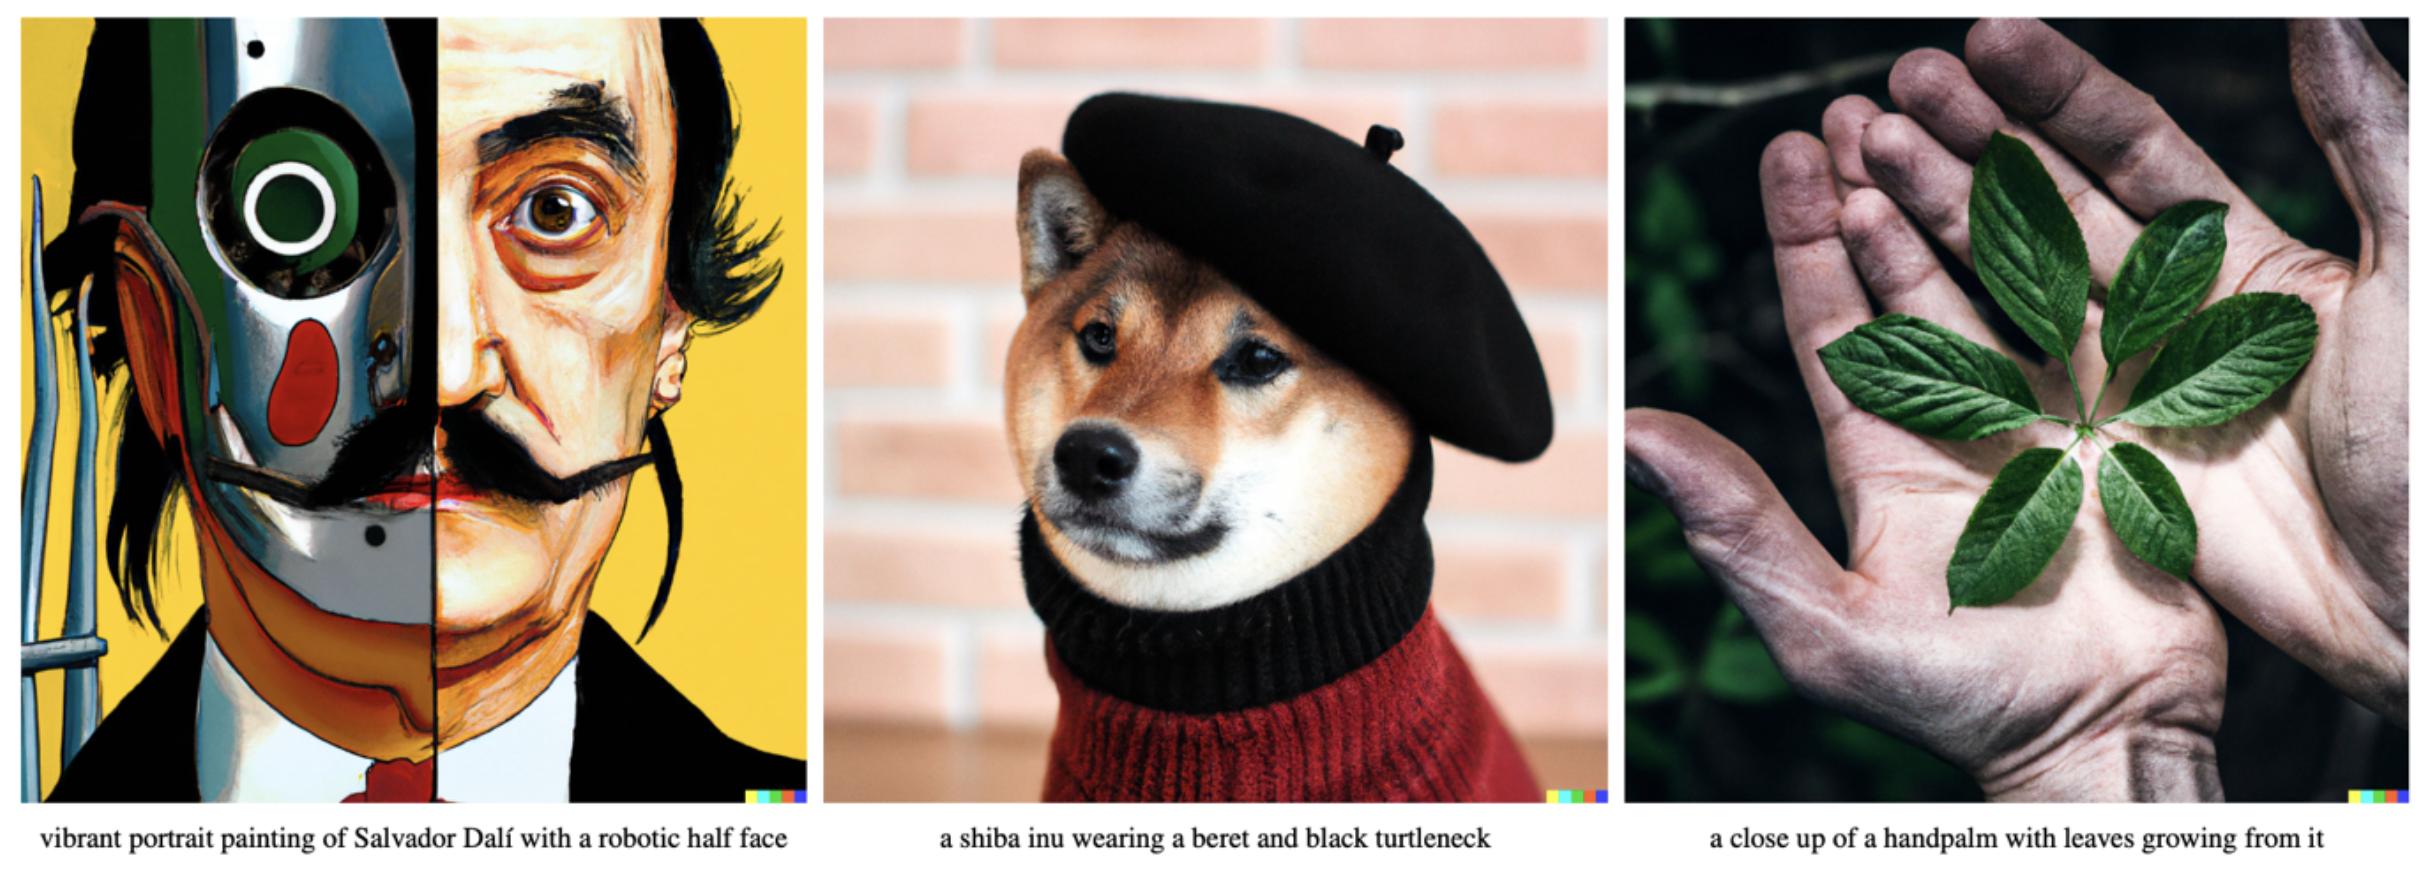
\includegraphics[width=1\textwidth]{Pictures/DallE2.png} 
    \caption{\textbf{Sample of generated images by DALL-E 2}. The images are of a quality and level of detail that are suitable for use in real-life scenarios. \cite{ramesh2022hierarchical}}
    \label{fig:DallE2}
\end{figure}

The generated images, as shown in figure \ref{fig:DallE2}, are of high enough quality to be used in real-world projects. Hence, research has shifted from concentrating solely on the quality aspect to trying to increase control over the final result. Therefore, in late 2022 and early 2023, some of the most influential publications in the field of generative AI seek to facilitate the manipulation of generated images through \textit{subject-driven generation} (\textit{\textit{An Image is Worth One Word: Personalizing Text-to-Image Generation using Textual Inversion}} \cite{gal2022image} and \textit{DreamBooth: Fine Tuning Text-to-Image Diffusion Models for Subject-Driven Generation} \cite{ruiz2023dreambooth}) or conditional guidance (Adding Conditional Control to Text-to-Image Diffusion Models \cite{zhang2023adding}).

\section{Diffusion probabilistic models} \label{Dprobabilistic}

Throughout 2022, the capabilities and popularity of text-to-image models have exploded. The general public is aware of some models, such as DALL-E 2, Midjourney, or Stable Diffusion. Nonetheless, the vast majority of people are unaware of the technical prowess required in the field of Artificial Intelligence for these models to exist. This section aims to shed some light on the internal functioning and processes of these models from an academic perspective.

\textit{Diffusion probabilistic models} are a class of latent variable models that introduce the ideas of nonequilibrium thermodynamics into data generation techniques by homogeneously adding noise into samples. Thus, they join the list of models that manage to generate high-quality images, such as variational autoencoders (VAEs) or Generative adversarial networks (GANs). The latter ones have been the reference of academic research in recent years and are the benchmark to be surpassed by \textit{diffusion models}. 

GANs were introduced in 2014 by researchers at the University of Montreal in the paper \textit{Generative Adversarial Nets} \cite{goodfellow2020generative}. The idea is to create generative models through an adversarial process in which two neural networks compete against each other.  One of the networks will be generative while the other will be discriminative. Thus, the generative network will be in charge of capturing the distribution of the training dataset while the discriminative network must distinguish whether a sample comes from the generative network or the training data. The idea is that the generative network maximises the probability that the discriminative network makes errors. 

\textit{Diffusion models}, on the other hand, achieve high-quality image synthesis results in the paper \textit{Denoising Diffusion Probabilistic Models} \cite{ho2020denoising} by researchers from the University of California, Berkeley. These models are based on creating a Markov chain in which at each step they add Gaussian noise to an image in a diffusion process and then learn to undo it. In this way, a network is trained that is capable of reconstructing images from random noise. The differences between GANs and \textit{diffusion models} are presented in figure \ref{fig:GansvsDM}.

\begin{figure}
    \centering
    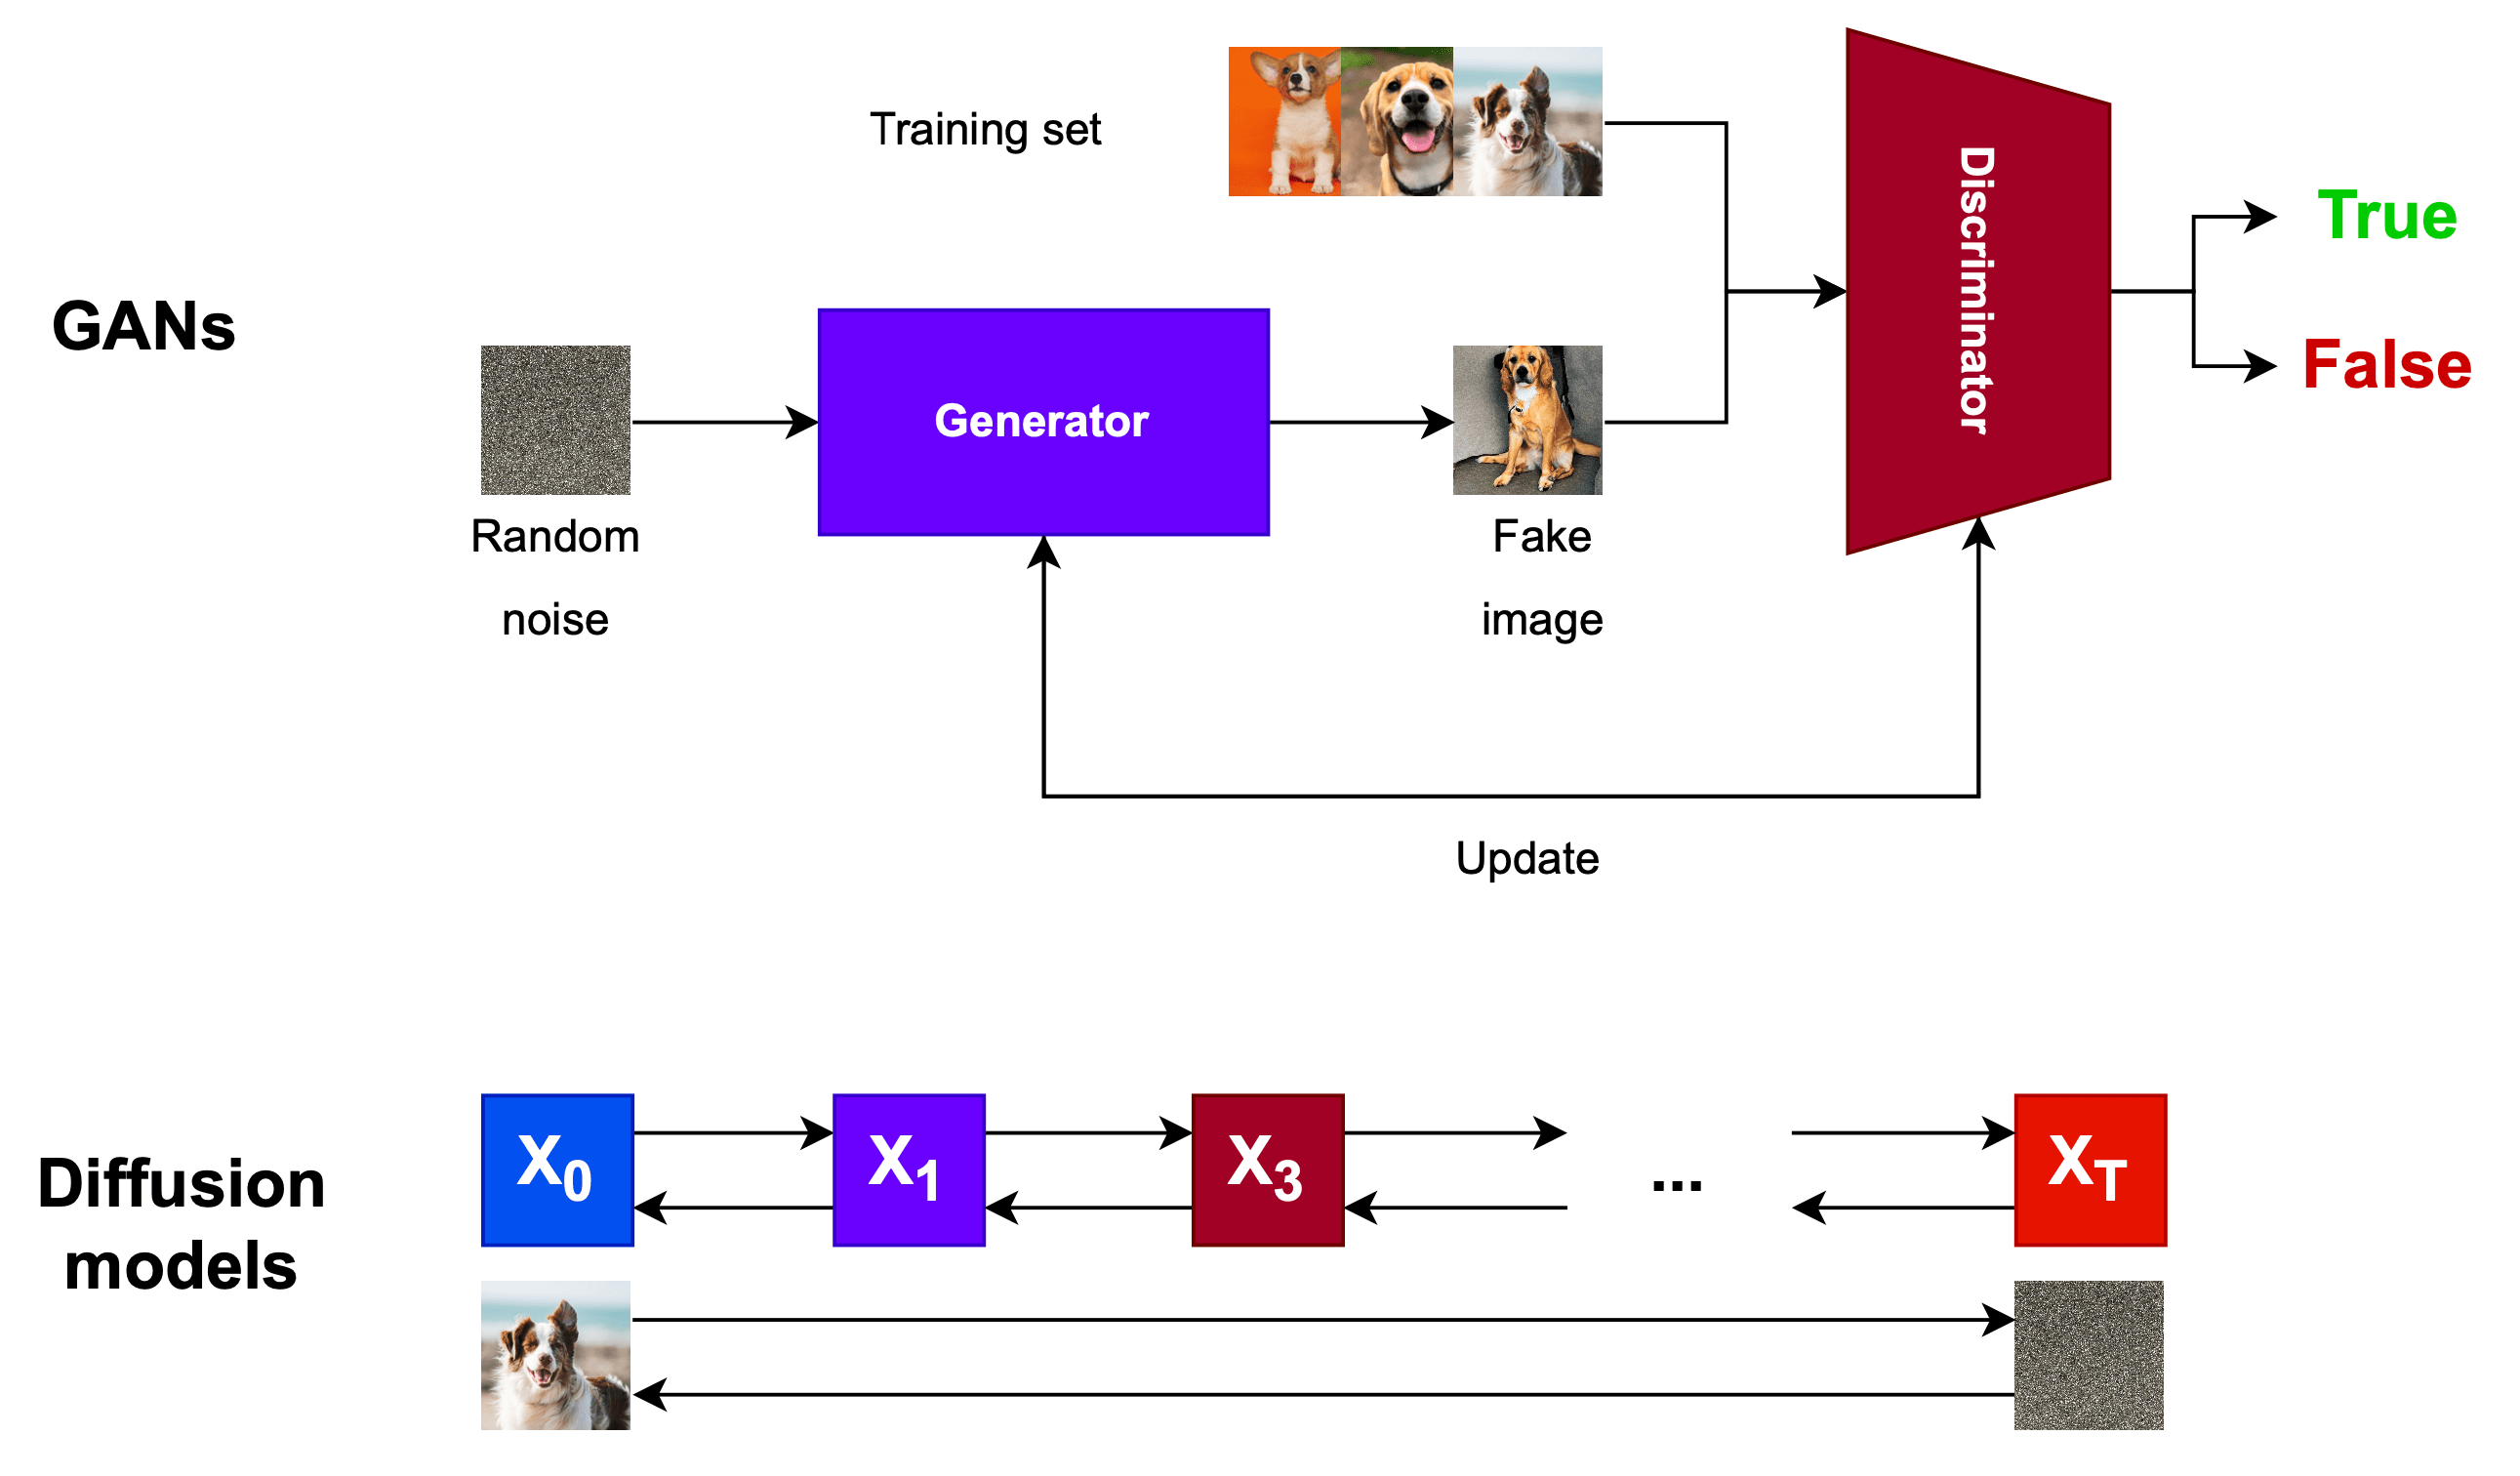
\includegraphics[width=1\textwidth]{Pictures/GansvsDM} 
    \caption{\textbf{Overview of GANs and diffusion models}. In GANs, a generative and a discriminative network compete with each other in a process that improves both at the same time. \textit{Diffusion models}, on the other hand, are based on a Markov chain that adds noise and then learns how to remove it.}
    \label{fig:GansvsDM}
\end{figure}

Diving further into the workings of \textit{diffusion models}, we define the forward process of the Markov chain. The first step is to take a sample of the target data distribution, which we will call $X_0$, and add Gaussian noise in $T$ steps. The forward process is thus defined as a Markov chain in which the state of a sample at time $n$ depends only on the state at time $n-1$. Therefore, one can denote the distribution of any sample conditioned on the initial state $X_0$.

\[ q\left(x_{1:T}\middle| x_0\right)=\prod_{t=1}^{T}{q\left(x_t\middle| x_{t-1}\right)} \]

In every step of the noising process, Gaussian noise is added according to some variance schedule $\beta_1...\beta_t$, normally consider as hyperparameters. The restrictions applied to $\beta_t$ are $\beta_1 < \beta_2 ... < \beta_t$ and $\beta_t \epsilon (0, 1)$. $I$ stands for identity.

\[q\left(x_t\middle| x_{t-1}\right)=\mathcal{N}\left(x_t;\sqrt{1-\beta_tx_{t-1}},\beta_tI\right) \]

As $\beta_t$ grows in time and $T$ approaches the limit ($T \rightarrow\infty$, $\beta_t \rightarrow 0$), the Gaussian mean will approach zero with identity covariance. In this way, the distribution will lose all the information contained in the original image. In practice, researchers use a $T$ close to 1000 \cite{ho2020denoising}.

\[q\left(x_t\middle| x_0\right)\approx\mathcal{N}\left(0,I\right)\]

Figure \ref{fig:MarkovchainDP} shows the diffusion process described so far.

\begin{figure}
    \centering
    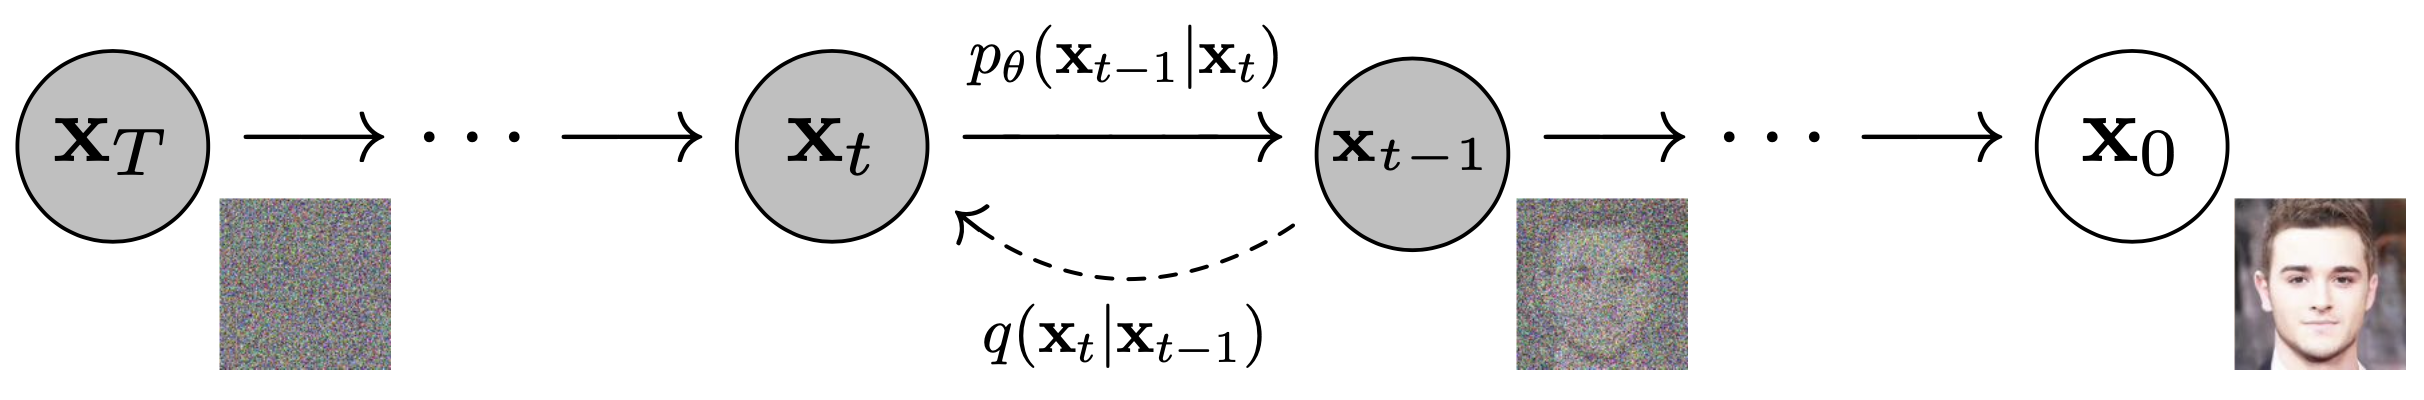
\includegraphics[width=1\textwidth]{Pictures/MarkovchainDP} 
    \caption{\textbf{Markov chain of the diffusion process} \cite{ho2020denoising}. As $T$ approaches the limit, the distribution will lose all the information of the original picture.}
    \label{fig:MarkovchainDP}
\end{figure}

In summary, it is proven that the forward process destroys the structure of a data distribution step by step. The next challenge is to learn the \textit{reverse diffusion process} in order to generate data that resembles the training distribution from pure Gaussian noise. As with the forward process, the \textit{reverse diffusion process} can be expressed as a Markov chain where the probability of a sequence of samples can be expressed as the product of conditional probabilities.

\[ p_\theta\left(x_{0:T}\right) := p\left ( x_T \right ) \prod_{t=1}^{T}p_\theta\left ( x_{t-1} | x_t\right ) \]

The \textit{reverse diffusion process} involves a neural network to remove noise from an image in a stepwise manner. Thus, starting from pure Gaussian noise, noise is removed step by step to arrive at an image that resembles the training distribution. The reason that the process has to be done in a stepwise manner is that ``the estimation is more tractable than explicitly describing the full distribution" as expressed in the publication \textit{Deep Unsupervised Learning using Nonequilibrium Thermodynamics} \cite{sohl2015deep}.

The neural network that the authors of DDPM propose aims to predict the noise to subsequently eliminate it from the image. This is equivalent to obtaining the mean of the distribution since the authors decide to fix the variance. The authors decide to use the U-Net network \cite{ronneberger2015u} for this purpose. U-Net consists of a bottleneck in the middle that ensures that the network removes irrelevant information and focuses on the important one. In addition, the network, between the encoder and the decoder, uses residual connections to improve efficiency. Finally, the authors of DDPM decide to employ self-attention at the 16 × 16 feature map resolution. Figure \ref{fig:ReverseDP} shows a schema of the learning process.

\begin{figure}
    \centering
    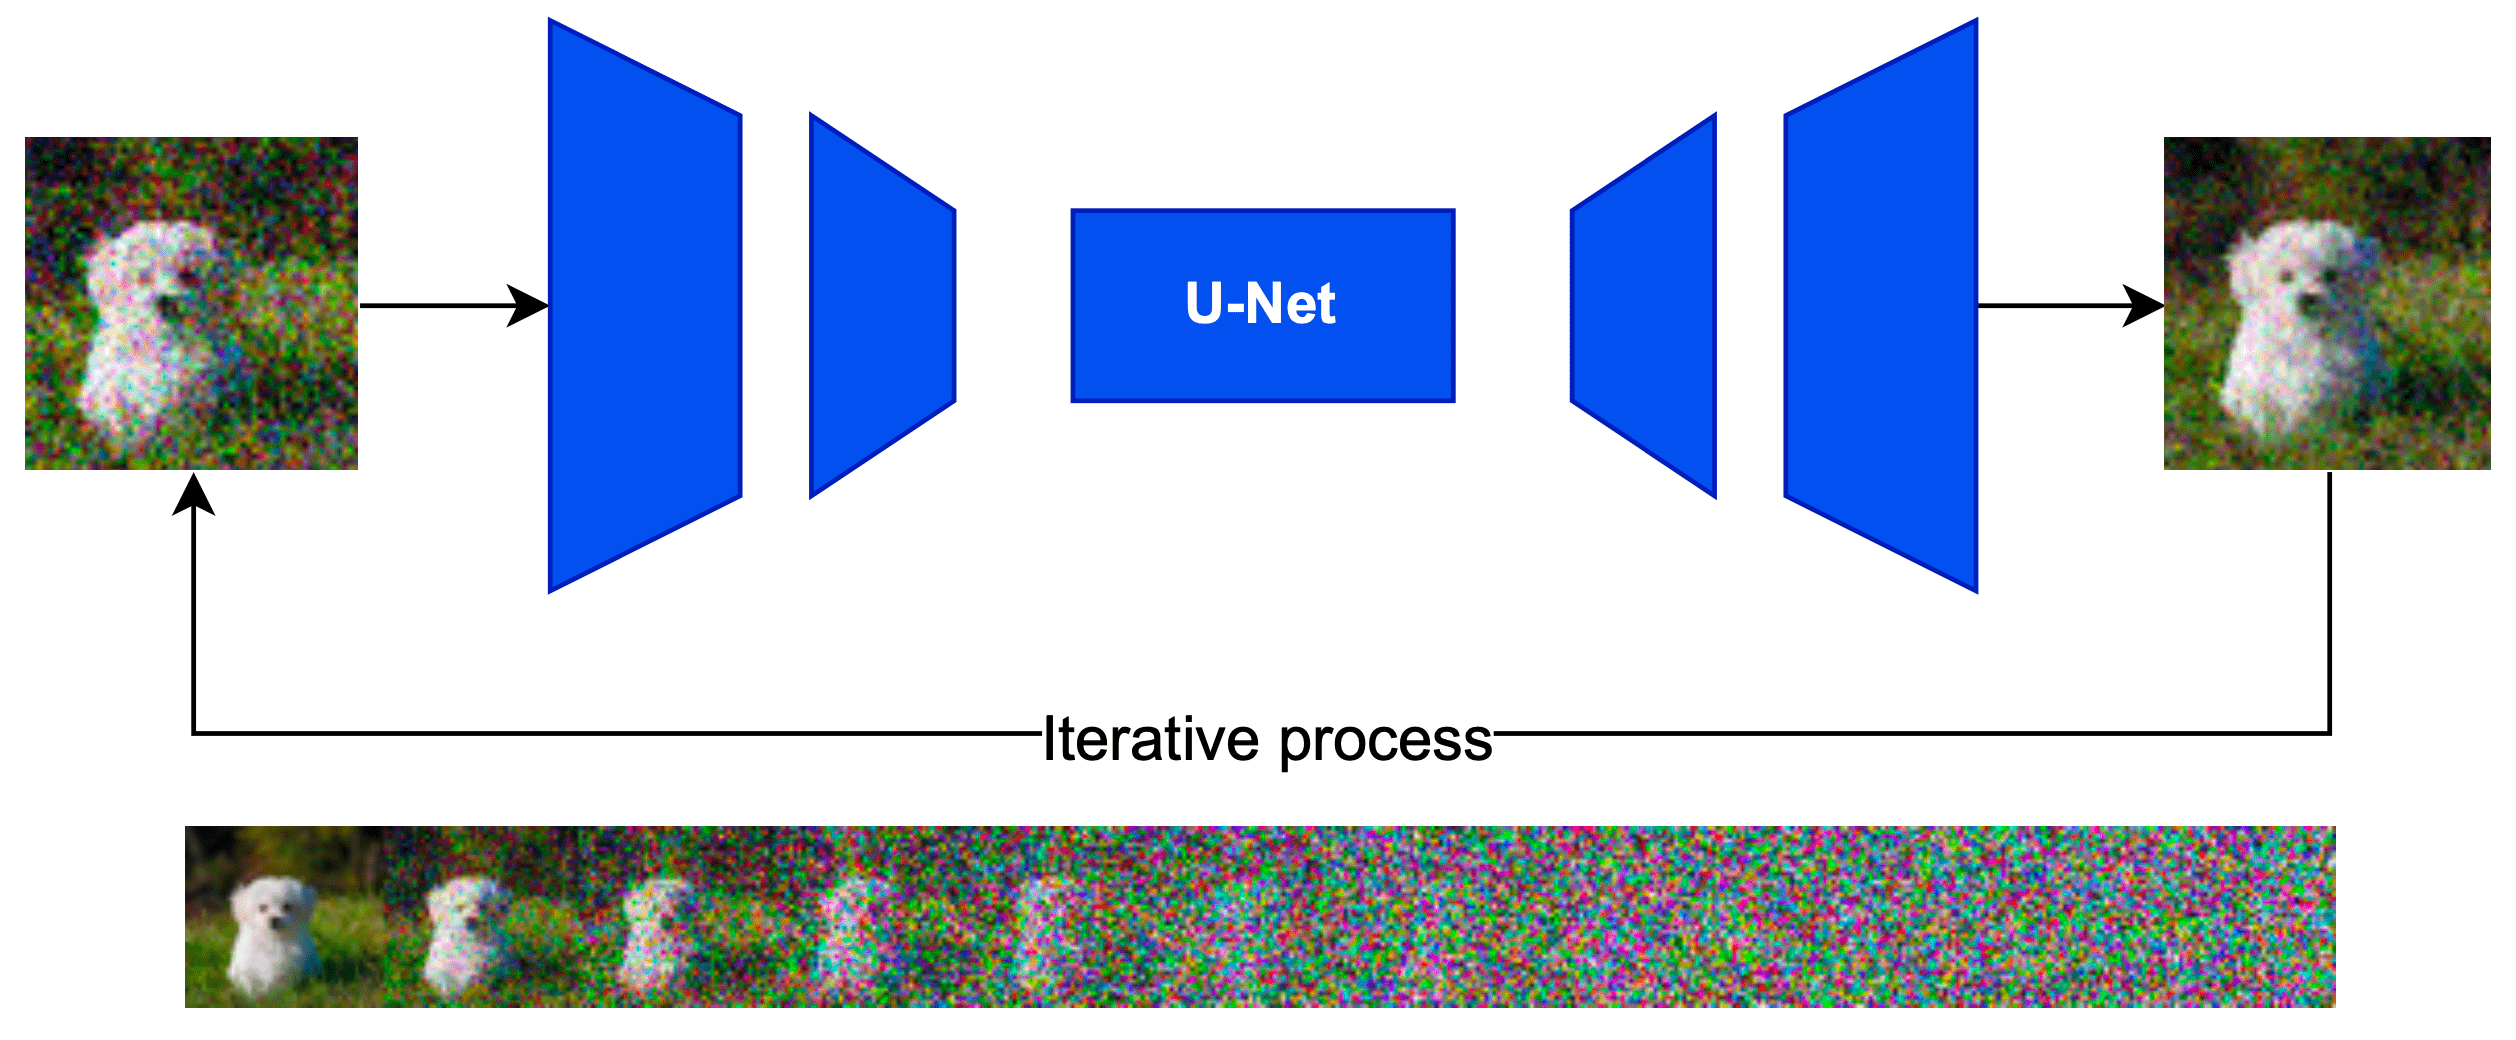
\includegraphics[width=0.8\textwidth]{Pictures/ReverseDP.png} 
    \caption{\textbf{Reverse diffusion learning schema}. The network is in charge of predicting the noise. Afterwards, it is eliminated from the image.}
    \label{fig:ReverseDP}
\end{figure}

Another question that arises when working with \textit{diffusion models} is how conditional generations can be provided. This can be achieved through various techniques. One way is to feed a conditional variable into the training so that the model makes use of it in the generation to resemble a subset of the training distribution. However, guiding the generation process through a classifier is a more flexible technique that allows even more complex text descriptions than simple labels to be worked with. The idea is to take an already trained classifier and guide the generation in the direction of the gradient of the classifier label.

\subsection{Improvements to diffusion probabilistic models }

Although the results obtained by the \textit{Denoising Diffusion Probabilistic Models} \cite{ho2020denoising} paper are excellent and represent a great leap forward compared to the images that the generative models were capable of producing until then, researchers at OpenAI suggest some improvements that increase the quality of the results in their publication \textit{Improved Denoising Diffusion Probabilistic Models} \cite{nichol2021improved}. In it, the main improvements they propose to the model are \textit{(i) the incorporation of learned variances and (ii) an improvement of the noise schedule}. 

As discussed in section \ref{Dprobabilistic}, the authors of the paper \textit{Denoising Diffusion Probabilistic Models} \cite{ho2020denoising} decided to fix the variance. However, the OpenAI researchers decide to learn the interpolation of the variance between an upper and lower bound. This allows them to maintain the quality of the samples and improve the log-likelihood. Finally, they modify the loss to depend on the variance by a \textit{scaling factor} $\lambda$ set experimentally to 0.001.

On the other hand, the OpenAI authors present a new noise schedule designed to be linear in the central region and have little change at the beginning and end. It is defined through $ \bar{\alpha_t}$, affecting the definition of the variances $\beta_t$ as follows.

\[\beta_t = 1 - \frac{\bar{\alpha}_t}{\bar{\alpha}_{t-1}}\]

The proposed cosine noise schedule can be seen in figure \ref{fig:CosineSC}. Whereas, figure \ref{fig:CosineEX} shows how each of the schedules adds noise to the image. The linear schedule destroys the information faster and presents a sub-optimal behaviour since the last steps are practically pure noise. Thus, the cosine schedule is superior as it allows a more controlled addition of noise.

\begin{figure}
    \centering
    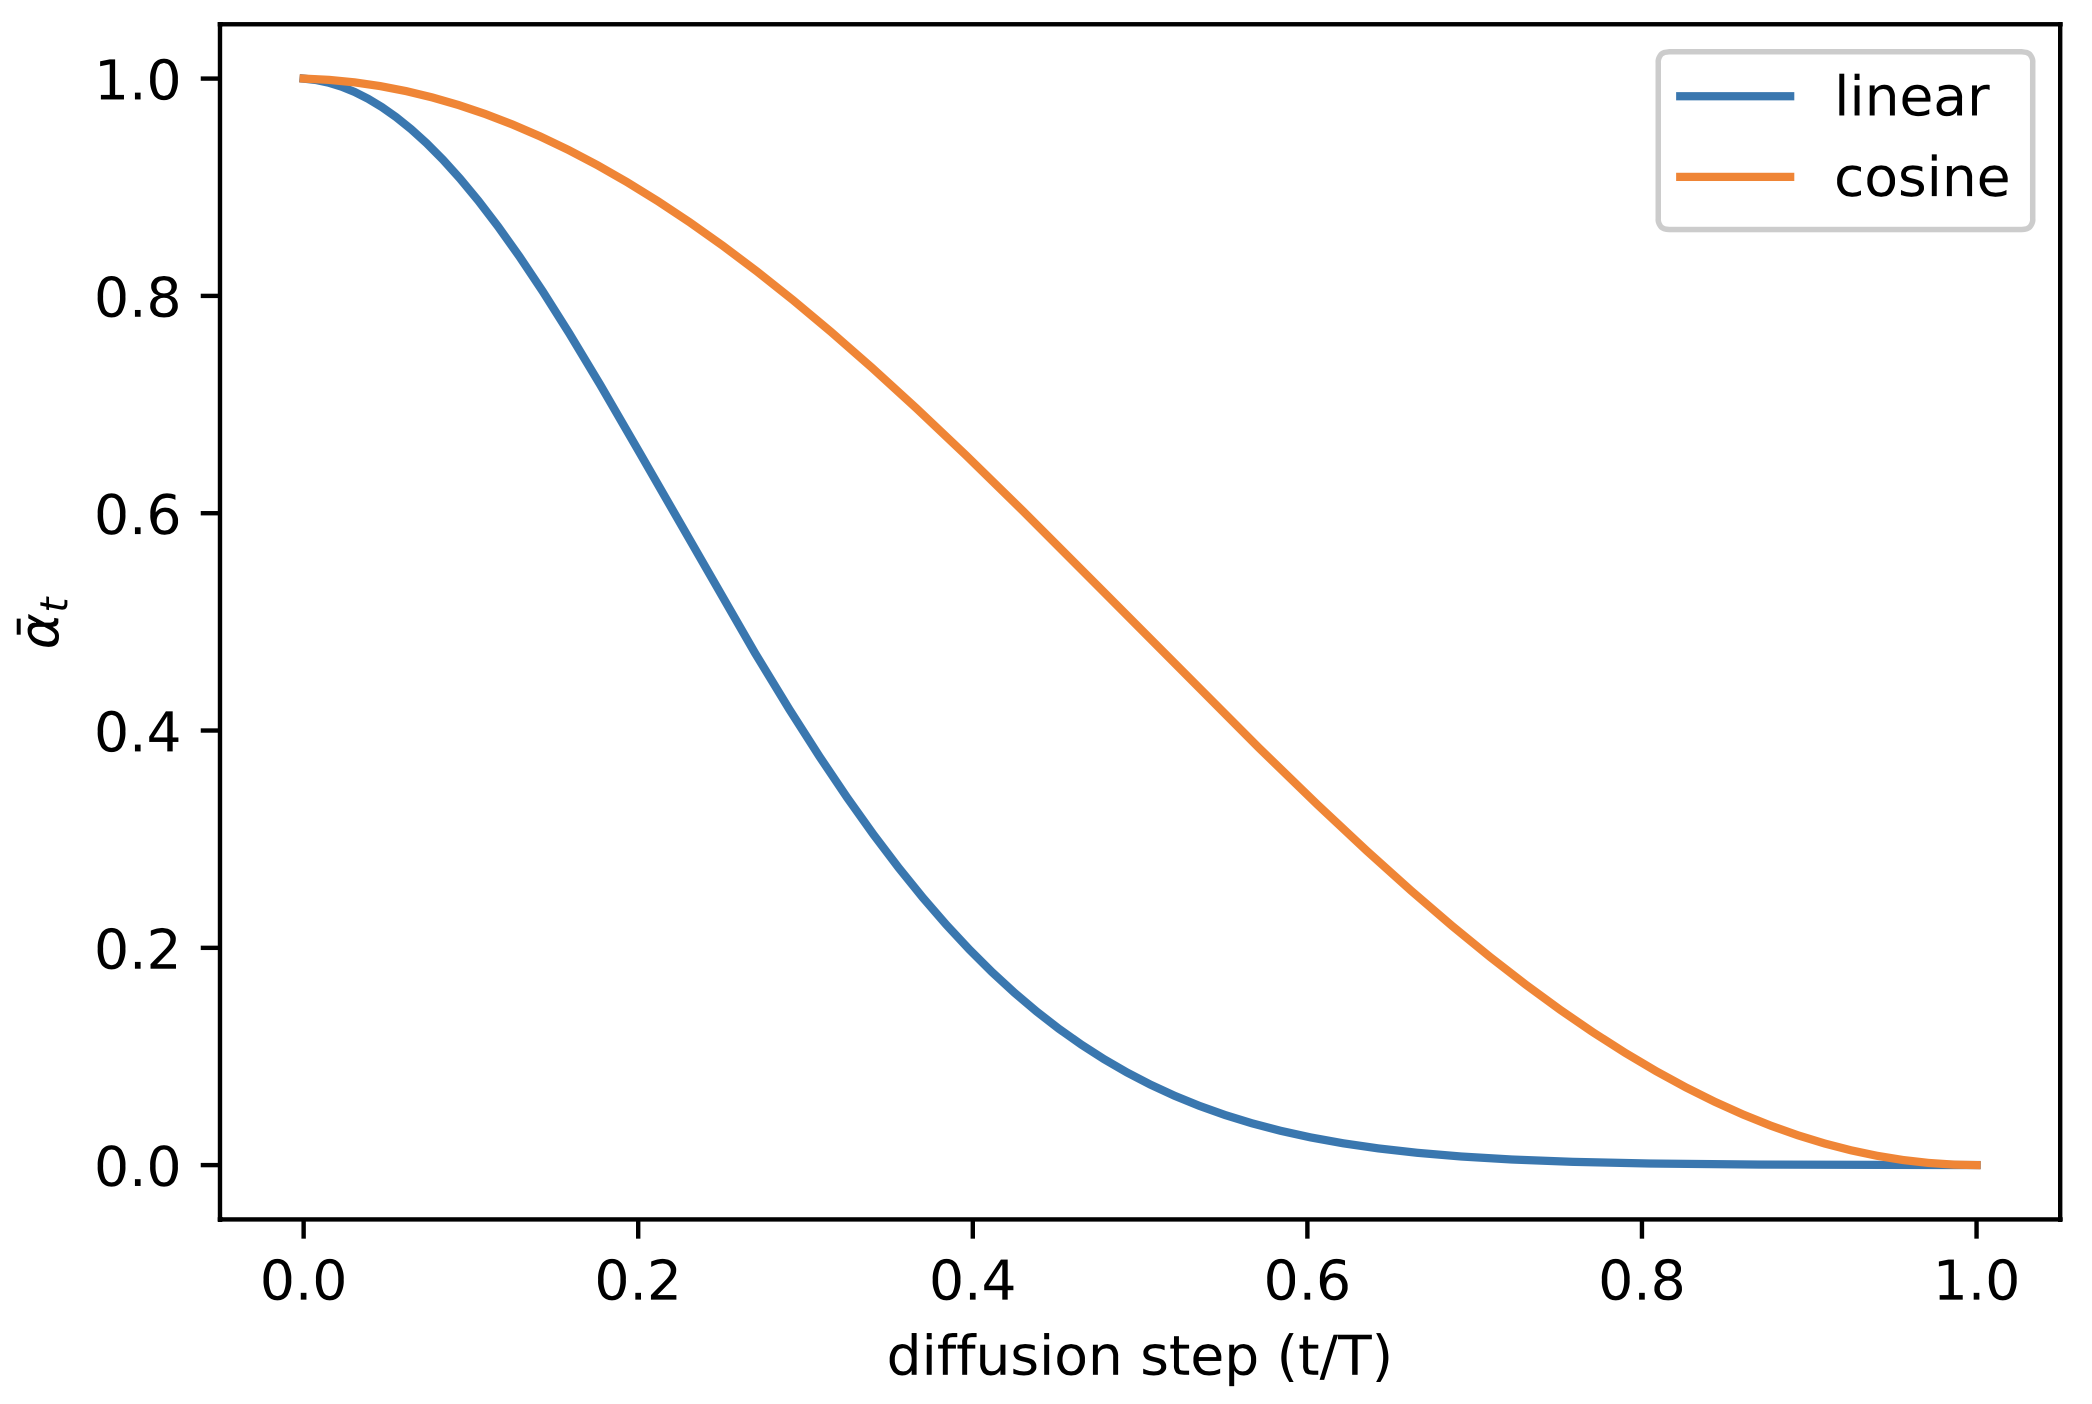
\includegraphics[width=0.50\textwidth]{Pictures/cosineSC.png} 
    \caption{\textbf{Cosine and linear schedules comparison }\cite{nichol2021improved}. The cosine schedule is designed to be linear in the central region and have little change at the beginning and end.}
    \label{fig:CosineSC}
\end{figure}

\begin{figure}
    \centering
    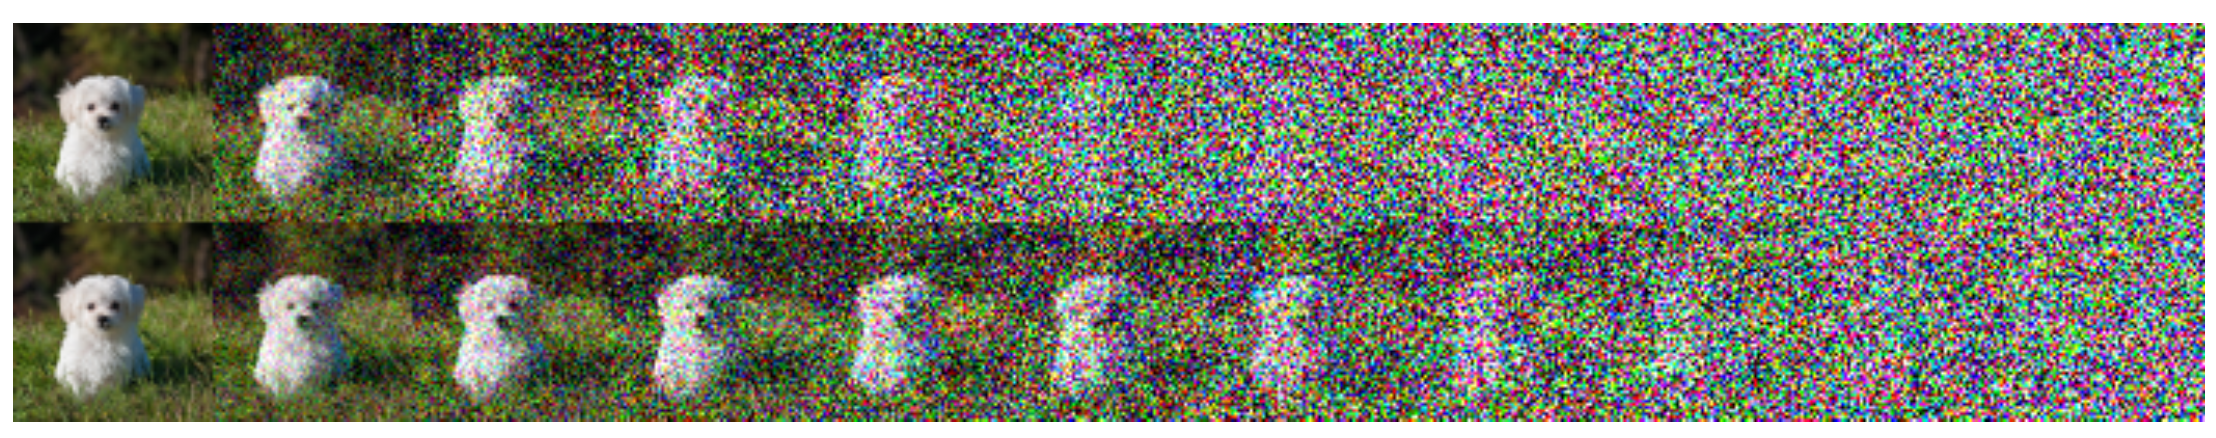
\includegraphics[width=0.75\textwidth]{Pictures/cosineEX.png} 
    \caption{\textbf{Cosine (bottom) and linear (top) schedules comparison on an image} \cite{nichol2021improved}. Cosine schedule allows a more controlled addition of noise. Thus, it avoids that last steps are practically pure noise.}
    \label{fig:CosineEX}
\end{figure}

However, the improvements do not stop there. The same OpenAI researchers in a later paper called \textit{Diffusion Models Beat GANs on Image Synthesis} \cite{dhariwal2021diffusion} demonstrate how a series of modifications to the architecture and the use of \textit{classifier guidance} can produce images that are better than the state-of-the-art at the time. The enhancement they make to the architecture are:

\begin{itemize}
    \item Increasing the depth while decreasing the width to keep the size of the model relatively constant.
    \item Increased use of \textit{attention heads and layers}
    \item Upsampling and downsampling the activations by means of the \textit{BigGAN residual blocks} \cite{brock2018large}.
    \item Use of \textit{adaptive group normalization} (AdaGN) layers, in which the concept of group normalization is expanded by adjusting the normalization parameters of each group separately according to the input data.
    \item \textit{Classifier guidance}. Employing an additional classifier, the diffusion model is assisted in generating a certain class.
\end{itemize}

\section{Latent diffusion models} \label{Ldiffusion}

\textit{Probabilistic diffusion models} have enabled the generation of high-quality images with state-of-the-art results. However, they have a fundamental weakness that the successive iterations of improvements did not resolve. The fact that they operate in pixel space, dealing with additions and deletions of noise in a tensor of the same size as the input tensor, means that training these models requires enormous computational resources. Therefore, researchers from the Ludwig Maximilian University of Munich and Runway ML propose in the publication \textit{High-Resolution Image Synthesis with Latent Diffusion Models} \cite{rombach2022high} to use \textit{latent space} instead of pixel space to speed up the training and inference calculations of these models. The \textit{latent space} is obtained from previously trained autoencoders, thus obtaining a representation of the images in a lower dimensional space that allows a balance to be reached between the quality of the details preserved and the reduction of the complexity obtained.

\begin{figure}
    \centering
    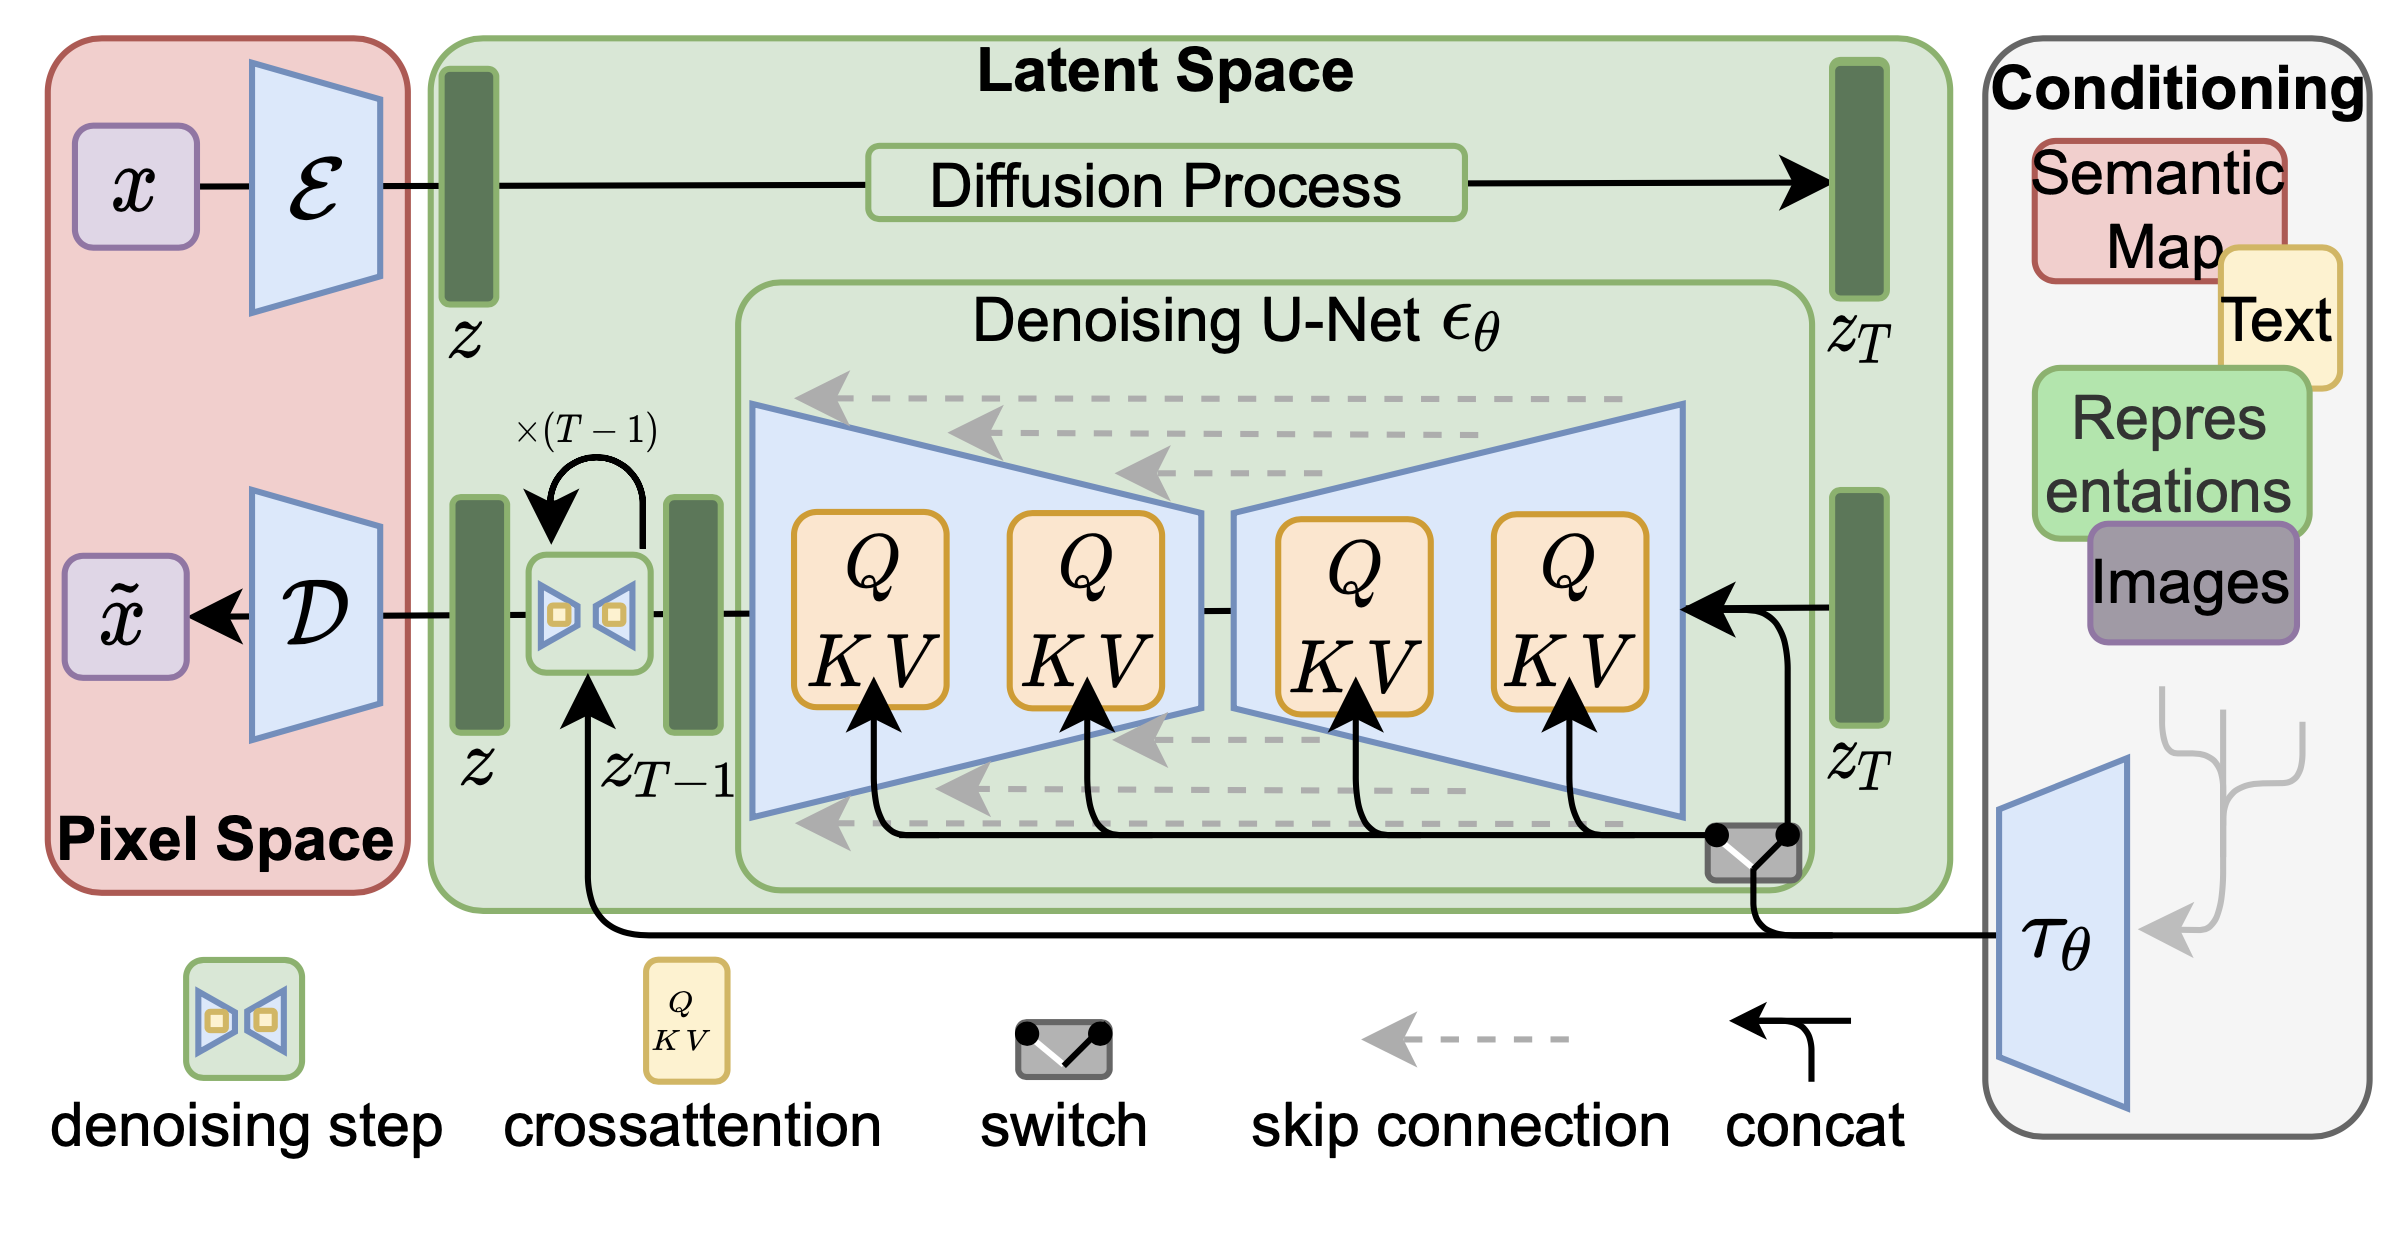
\includegraphics[width=1\textwidth]{Pictures/LDMDiagram.png} 
    \caption{\textbf{Latent diffusion architecture} \cite{rombach2022high}. First, a representation of the image in the latent space is obtained. Then, Gaussian noise is added to the diffusion process. For the inverse process, a U-Net network is used. Meanwhile, the encoder $\tau_\theta$ maps the conditionings. Ultimately, the result of the latent space is returned to the pixel space.}
    \label{fig:LDMDiagram}
\end{figure}

Thus, the operation of latent diffusion models can be summarised in the diagram present in figure \ref{fig:LDMDiagram}. The first training step is to obtain a representation of the considered image in the \textit{latent space} $\mathcal{Z}$ thanks to the encoder  $\mathcal{E}$. Then, Gaussian noise is added to the \textit{diffusion process} until $\mathcal{Z}_t$ is reached. For the inverse process, a U-Net network is used. However, the real strength of this approach lies in the ability to condition the generation. This is achieved thanks to a dedicated encoder $\tau_\theta$ that maps the conditionings in the intermediate layers of the U-Net with cross-attention layers. Finally, the result of the \textit{latent space} is returned to the pixel space thanks to the $\mathcal{D}$ decoder.

\section{Stable diffusion} \label{SD}

As detailed in section \ref{Hreview}, text-to-image models have exploded in popularity and capabilities throughout 2022. One of the biggest drivers of this shift in public perception has been Stable Diffusion, an \textit{open-source} model whose weights and architecture have been publicly released. As a consequence, many researchers and enthusiasts have put much effort into optimising and extending the project's capabilities. These efforts are led by the British generative AI startup Stability AI. As a result of the \textit{open-source} philosophy, this model is capable of running on consumer-available hardware. This fact allows the community to leverage its capabilities in a wide variety of cases.

Stable Diffusion is a latent diffusion model that follows the architecture developed by the Computer Vision \& Learning group of the Ludwig Maximilian University of Munich in the paper \textit{High-Resolution Image Synthesis with Latent Diffusion Models} \cite{rombach2022high}, which has already been explained in section \ref{Ldiffusion}. The proposed technique can also be adapted to other tasks such as \textit{inpainting, outpainting}, generating image-to-image translations or increasing the resolution of an image, all tasks that Stable Diffusion can perform. A high-level diagram of the main components of the model can be seen in figure \ref{fig:SDdiagram}:

\begin{figure}
    \centering
    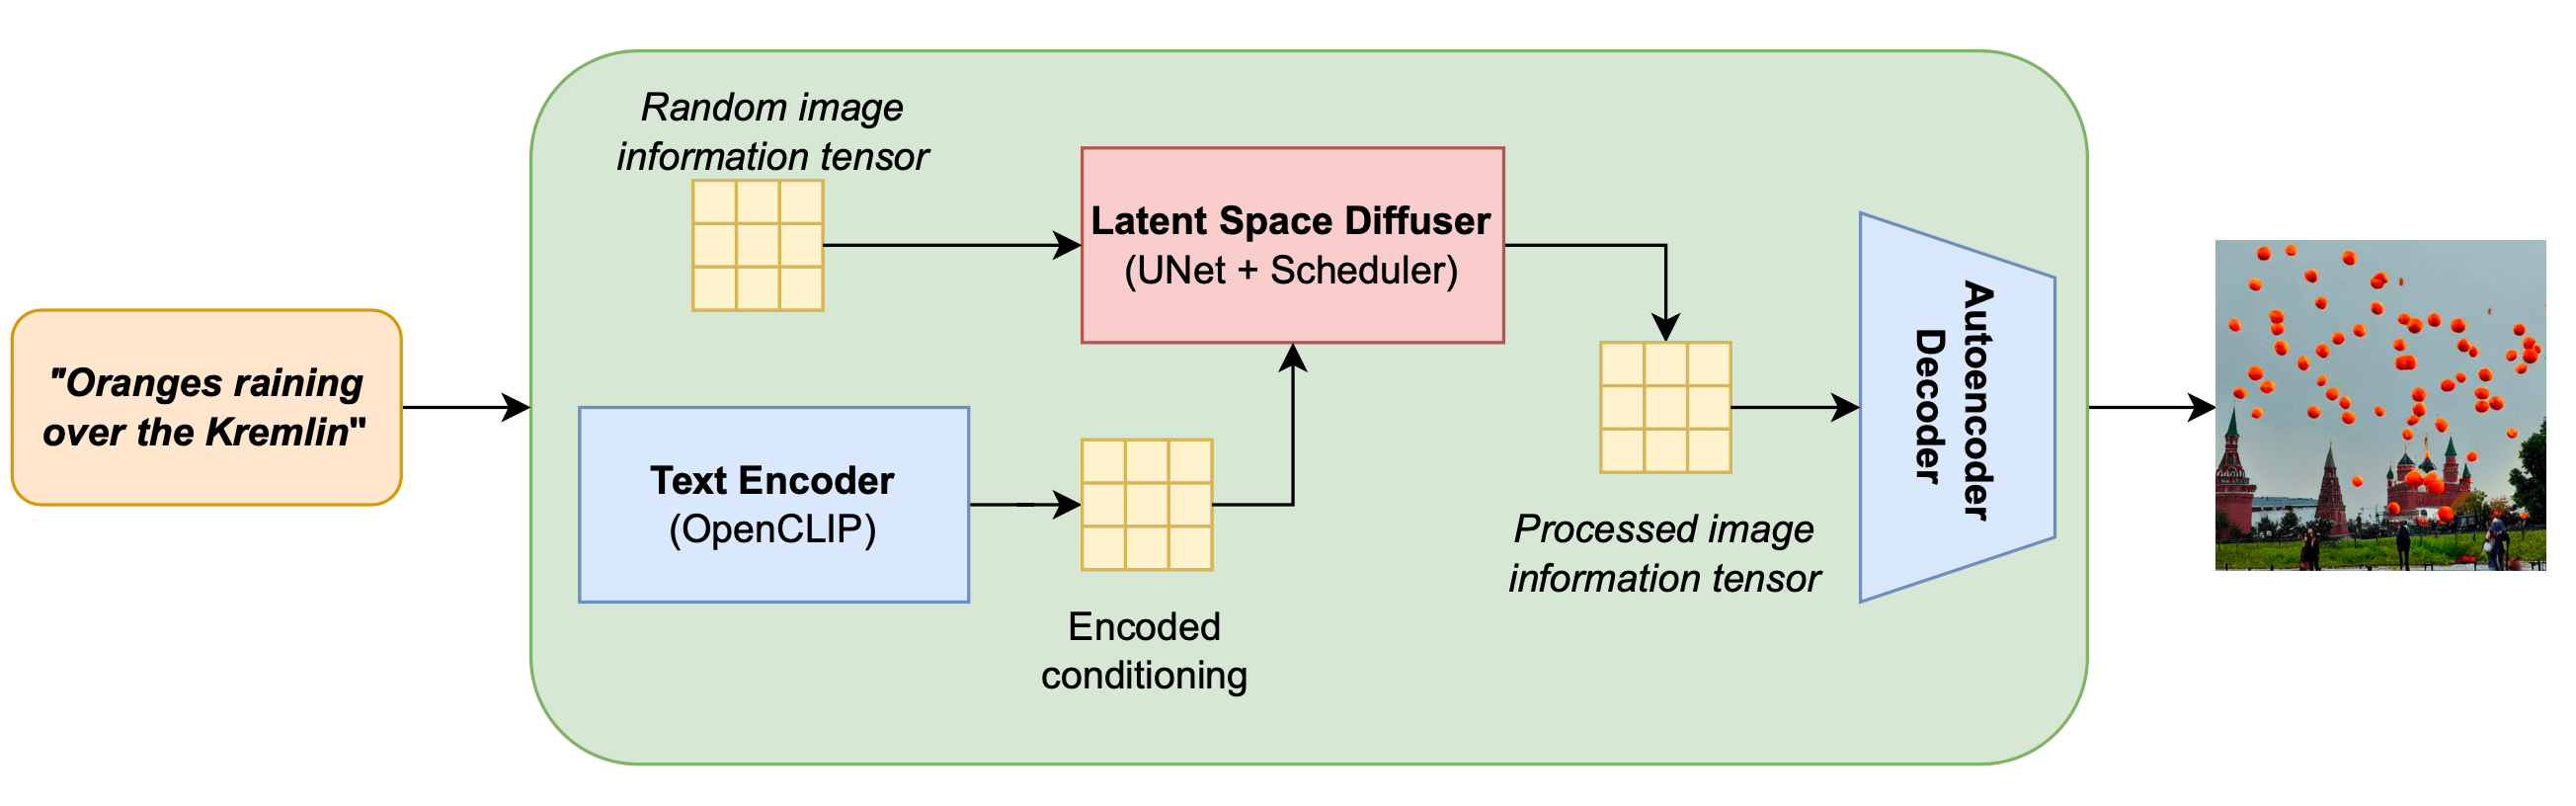
\includegraphics[width=1\textwidth]{Pictures/SDdiagram.png} 
    \caption{\textbf{Stable Diffusion main components}. The text encoder produces the encoding of the description. The latent space diffuser applies the diffusion process into the latent space to remove the noise. Finally, the autoencoder decoder generates the final image in the pixel state.}
    \label{fig:SDdiagram}
\end{figure}

\begin{itemize}
    \item \textbf{Text Encoder}: It creates an encoded representation of the text data's description. Its goal is to influence the \textit{diffusion process}, ensuring that the resulting image corresponds to the given description. Stable Diffusion's first version utilizes CLIP \cite{radford2021learning}, while its second version includes OpenClip \cite{cherti2022reproducible}. In both cases, the text encoder is used in conjunction with an image encoder. CLIP and OpenClip strive to maximize the similarity between the two encodings, enabling the model to associate images with their respective descriptions.
    \item \textbf{Latent Space Diffuser}: It aims to utilize the \textit{diffusion process} to eliminate noise from the image by manipulating the latent space information. As the process progresses, additional information is added to enhance the similarity between the image and the provided description. It is crucial to highlight that this operation takes place in latent space, resulting in improved efficiency and being a key advancement. Figure \ref{fig:DProcess} provides a visual representation of the denoising process guided by the text encoder.
    \item \textbf{Autoencoder Decoder}: The final image is produced by utilizing the compressed information stored in the latent space. This step is carried out only once to construct the ultimate pixel image.
\end{itemize}

\begin{figure}
    \centering
    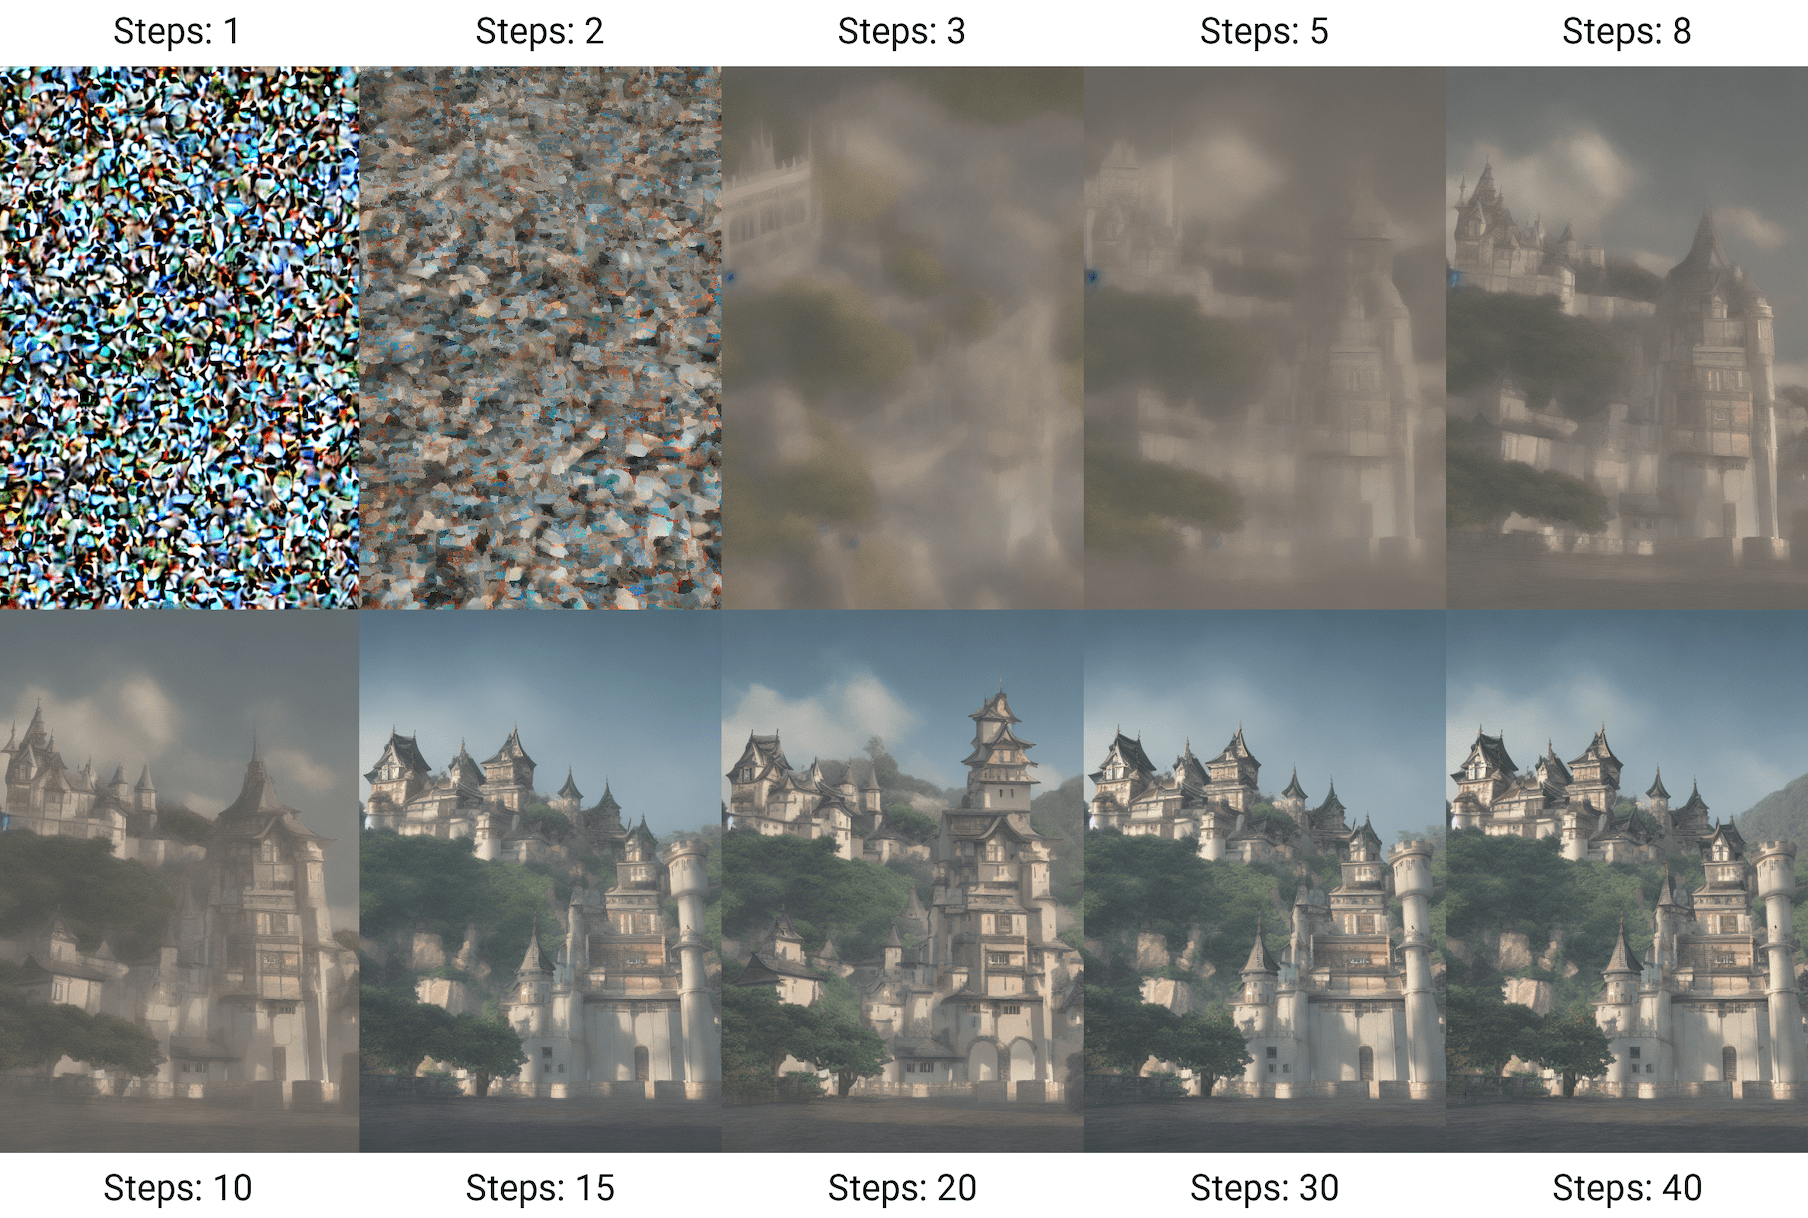
\includegraphics[width=1\textwidth]{Pictures/DProcess.png} 
    \caption{\textbf{Diffusion steps} \cite{wikiStableDiffusion}. The diffusion process is applied into the latent space to remove the noise.}
    \label{fig:DProcess}
\end{figure}

\subsection{Training dataset}

A significant challenge posed by models like Stable Diffusion is the choice of images they are trained on. This issue is not insignificant as image generation models require both textual descriptions of training images and a sufficient amount of variety to enable the model to comprehend how the world is constructed and thus be capable of reproducing it. However, the conventional datasets of the Machine Learning field (COCO, ImageNet, etc) fail to satisfy these requirements since they are not intended for this purpose. Researchers have discovered that the solution is the web, where a vast array of diverse images about the world can be found, many of which have HTML alt attribute tags.

Stable Diffusion has an advantage over some of its rivals, including \textit{DALL-E 2}, in that it is an \textit{open-source} project, meaning that the dataset employed for training is well-known and accessible to everyone. Specifically, the dataset used by Stable Diffusion is ``\textit{LAION-5B, a dataset of 5.85 billion CLIP-filtered image-text pairs, 14x larger than LAION-400M, previously the biggest openly accessible image-text dataset in the world}" \cite{schuhmann2022laion}. In particular, Stable Diffusion presents several checkpoints on various LAION-5B assemblies. Some of these checkpoints in Stable Diffusion version 1 \cite{SDCardHF} are:

\begin{itemize}
  \item \textbf{stable-diffusion-v1-1}: 256 x 256 images from a subset of 2.3 billion English-captioned images called LAION-2B-EN.
  \item \textbf{stable-diffusion-v1-2}: Resumed training on \textit{stable-diffusion-v1-1} with 512x512 images from the subset LAION-2B-EN, containing a selection of improved aesthetics images compared to the others.
  \item \textbf{stable-diffusion-v1-3}: Resumed training on \textit{stable-diffusion-v1-2} with the same subset of images but a 10\% dropping of the text-conditioning.
  \item \textbf{stable-diffusion-v1-4}: Resumed training on \textit{stable-diffusion-v1-2} with 512x512 images from the subset LAION-Aesthetics v2 5+, containing 600 million images from LAION-2B-EN with better aesthetics and low-resolution and watermarked images filtered out.
  \item \textbf{stable-diffusion-v1-5}: \textit{stable-diffusion-v1-4} trained with more steps.
\end{itemize}

LAION-5B retrieves images from the internet that are not uniformly high in quality. Because these images are gathered automatically, they do not adhere to the same rigorous standards as other image datasets. As a result, the checkpoints for training Stable Diffusion use varying subsets of LAION-5B. Nonetheless, the fact that the images obtained are not accurately labelled as they are in standard vision supervised learning is actually an advantage. Consequently, Stable Diffusion is now included in the group of architectures, such as CLIP or DALL-E 2, that have proven the value of these vast datasets, even though they contain a significant amount of noise.

LAION-5B contains 5.85 billion image-text pairs divided into three subsets. LAION2B-EN, which contains 2.32 billion English image-text pairs; LAION2B-MULTI with 2.26 billion image-text pairs from all other languages (Russian, French and German as top 3) and LAION1B-NOLANG of 1.27 billion samples where the language is not correctly defined. 

\subsubsection{LAION-5B Description}

The attributes that can be found in LAION-5B are described in table \ref{table:TableLaionAttributes}.

\begin{table}[ht]
\centering
\begin{tabular}{|p{0.25\linewidth} | p{0.69\linewidth}|}
\hline
\rowcolor[HTML]{AEAAAA} 
{\textbf{Attribute}} & {\textbf{Description}} \\ \hline
\textbf{id} & Image identifier \\ \hline
\textbf{URL} & URL from where the image was obtained \\ \hline
\textbf{Text string} & Caption accompanying the image \\ \hline
\textbf{Dimensions} & Height and width of the image \\ \hline
\textbf{Similarity} & Cosine similarity between the text and image embeddings. CLIP-based   models are employed to gauge the level of accuracy with which an image is   described by a given textual description.\\ \hline
\textbf{pwatermark} & Probability that the image presents a watermark. The value is   obtained by a custom model trained by LAION. Value between 0 and 1 \\ \hline
\textbf{punsafe} & Probability that the image is NSFW. As some of the content   acquired from the web may not be suitable for all audiences, LAION employs a   custom model to assess its adequateness. Value between 0 and 1 \\ \hline
\end{tabular}
\caption{\textbf{LAION-5B’s attributes}. Each of the images contained in the dataset has these defining attributes of quality and usability.}
\label{table:TableLaionAttributes}
\end{table}

Some statistics of the subsets computed by the LAION team can be found in table \ref{table:TableLaionStatistics} \cite{schuhmann2022laion}.

\begin{table}[ht]
\centering
\begin{tabular}{|l|p{0.24\linewidth}|l|l|p{0.25\linewidth}|}
\hline
\rowcolor[HTML]{AEAAAA} 
\textbf{Subset} & \textbf{Dimensions} & \textbf{NSFW} & \textbf{Watermark} & \textbf{Average text length} \\ \hline
\textit{2B-EN} & \begin{tabular}[c]{@{}l@{}}-   \textgreater{}256x256: 1324M\\    \\ -   \textgreater{}512x512: 488M\\    \\ -   \textgreater{}1024x1024: 76M\end{tabular} & 2.9\% & 6.1\% & 67 \\ \hline
\textit{2B-MULTI} & \begin{tabular}[c]{@{}l@{}}-   \textgreater{}256x256: 1299M\\    \\ -   \textgreater{}512x512: 480M\\    \\ -   \textgreater{}1024x1024: 57M\end{tabular} & 3.3\% & 5.6\% & 52 \\ \hline
\textit{1B-NOLANG} & \begin{tabular}[c]{@{}l@{}}- \textgreater{}256x256:   1324M\\    \\ -   \textgreater{}512x512: 488M\\    \\ -   \textgreater{}1024x1024: 76M\end{tabular} & 3\% & 4\% & 46 \\ \hline
\end{tabular}
\caption{\textbf{Statistics summary for LAION-5B}. NSFW and Watermark refer to the percentage of graphic and watermarked images while Average text length refers to the average length of the descriptions.}
\label{table:TableLaionStatistics}
\end{table}

By analysing the data presented in tables \ref{table:TableLaionAttributes} and \ref{table:TableLaionStatistics}, one can infer the rationale behind the various checkpoints employed in the Stable Diffusion model. The LAION-5B dataset, owing to its extensive diversity, can be partitioned into subsets that cater to various generation objectives. As a result, the model can be adapted to different resolutions or the quality of the generated images can be adjusted by filtering out low similarity image-to-description pairs, NSFW content, or watermarked content.

It is noteworthy to mention that the primary characteristics of the entries in the dataset are produced by other pre-trained models. This highlights the significance of incorporating other models in the data collection process for large AI models, as they can assist in adding supplementary features to the dataset. A more detailed discussion of this fact can be found in section \ref{LCollection}

\subsubsection{LAION-5B Collection Methodology} \label{LCollection}

The pipeline followed when creating the LAION-5B dataset involves: (i) obtaining Common Crawl data, (ii) filtering some web pages, (iii) downloading the image-text pairs, (iv) and filtering the content according to various characteristics.

Common Crawl is an organization dedicated to web crawling, data collection, and storage. It makes all the gathered data publicly available. In the October 2022 crawl, the total file size was 380 TBs, comprising 3.15 billion web pages. The dataset's key feature is that it contains HTML tag information about the images, including the ``\textit{alt}" attribute, which provides an alternative description of the images. This attribute is widely used on the web, for example, to address page rendering issues, assist visually impaired individuals, or aid web content indexing by search engines. Therefore, it is a ubiquitous attribute on the web that is encouraged to improve page usability and ranking in web search engines.

After the Common Crawl data is accessible, images that have information in the ``\textit{alt}" attribute are chosen. Once both images and descriptions are available, a language detection model is employed on the descriptions, and the data is then divided into three subsets: LAION2B-EN, LAION2B-MULTI, and LAION1B-NOLANG, as mentioned earlier. It is noteworthy that in order to incorporate data into LAION1B-NOLANG, a confidence threshold is determined based on the prediction of the language detection model, and if it is insufficient, it is included in this subset.

The next step is to clean the dataset of poor-quality images and descriptions. For this purpose, images, and descriptions with less than 5KB data, 5 words and 0.28 cosine similarity (in LAION2B-EN) are removed. The cosine similarity is computed thanks to Open AI's CLIP model, which computes the embedding of images and text.

It is important to notice the importance of the CLIP contrastive model in understanding how the Stable Diffusion training dataset was created. As explained above, CLIP is able to associate images and text. The way in which it achieves this is very clever as it can solve the classic problem of labels in deep learning. Thus, CLIP is a pioneer in bringing together language models and vision models by making supervision in natural language. And therein lies the key to LAION-5B: unlike other datasets that require a specialized team to create carefully curated tags, this dataset relies on natural language descriptions provided by internet users. This allows for much faster scalability. It is worth noting that CLIP is not only essential in the creation of the dataset, but it also plays a vital role in the Stable Diffusion model, as previously explained in section \ref{SD}.

The final stage of the pipeline involves incorporating additional attributes that help categorize the image in a useful way, beyond just its similarity to text. One such attribute is the probability that the image contains NSFW content, which is determined using a custom model. Another attribute is the probability that the image has a watermark, which is determined using a separate model designed for that purpose.

Summing up, the creation of LAION-5B relies on multiple AI models that help gather reliable content from the internet and guarantee the accuracy of image descriptions. This marks a significant shift in the way we collect data for training models, where the emphasis is on scaling the dataset rather than carefully generating accurate labels. Instead, models like CLIP enable the use of natural language descriptions that accompany web images for data collection.

\section{Subject-driven generation techniques}

Text-to-image models have enabled the generation of high-quality, realistic images through a textual description of the desired image, as discussed in sections \ref{Dprobabilistic}, \ref{Ldiffusion}, \ref{SD}. If we take, for example, Stable Diffusion and want to create an image of a specific subject or object, we will not be able to obtain the specific details that characterise it. The reason is that even if we perform multiple iterations on a prompt with a very detailed description of what we want to generate, the variability of the model will prevent us from reconstructing its key visual characteristics. Consequently, a new problem arises, \textit{subject-driven generation}. It consists of reconstructing a subject in different contexts while being able to maintain its characteristics and details. Figure \ref{fig:subjectD} depicts the subject-driven generation problem. The target is to create images of a specific subject in different contexts.

\begin{figure}
    \centering
    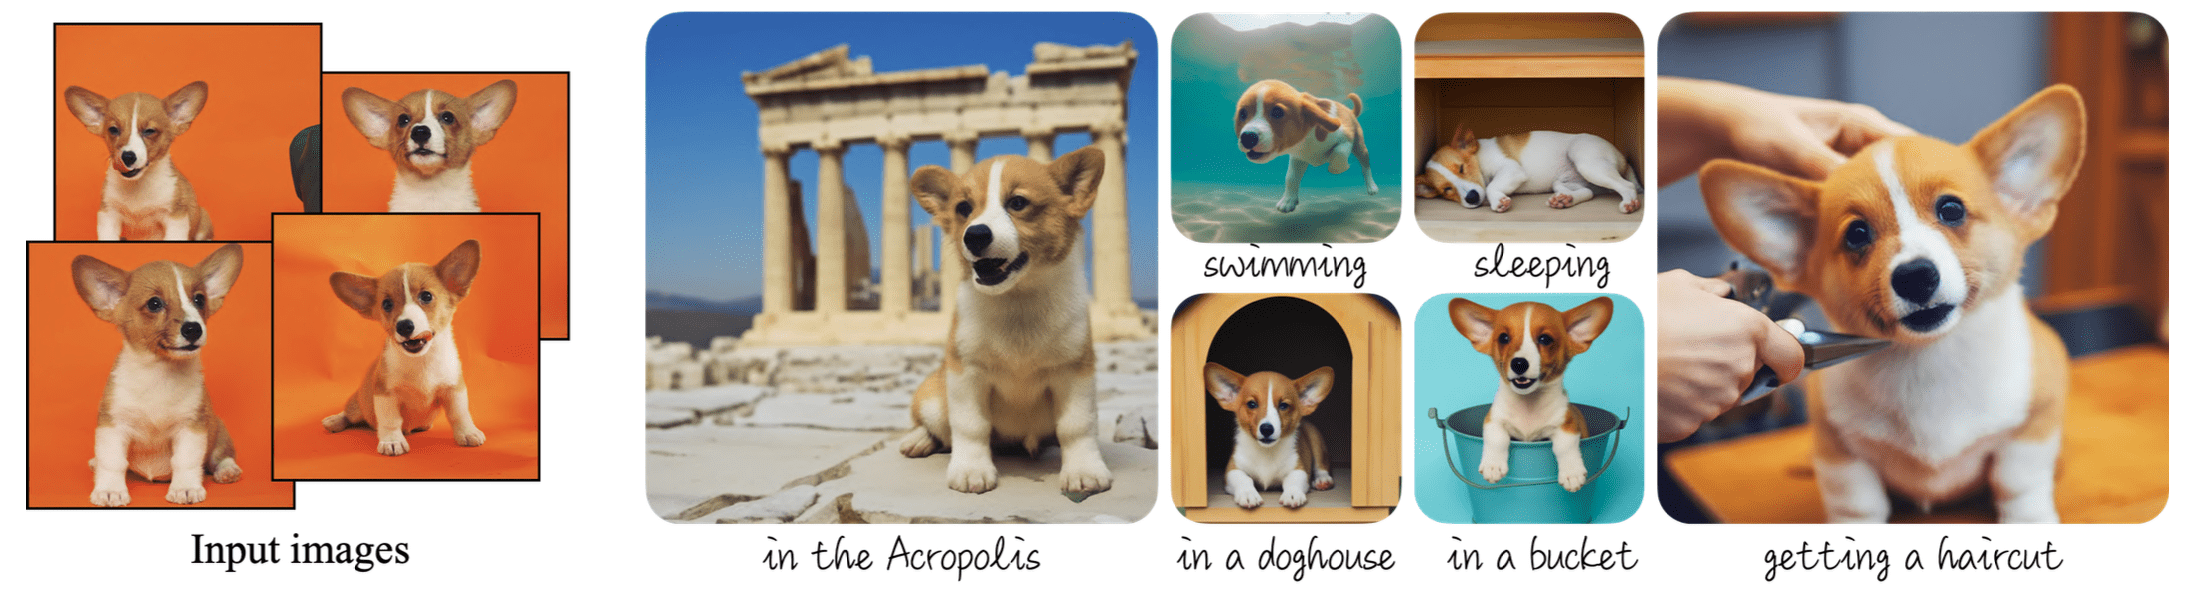
\includegraphics[width=0.9\textwidth]{Pictures/subjectD.png} 
    \caption{\textbf{Subject-driven generation problem} \cite{ruiz2023dreambooth}. The target is to create images of a specific subject in different contexts.}
    \label{fig:subjectD}
\end{figure}

On the other hand, in deep learning, it has been shown that the way forward is not to train models from scratch for each task. On the contrary, the way forward for research in recent years is to use transfer learning techniques to exploit the capabilities of the gigantic models already created and, in this way, to be environmentally responsible and avoid having to handle colossal datasets as training data \cite{zhuang2020comprehensive}.

For these reasons, the community is exploring the \textit{subject-driven generation} problem in depth. Among the proposed solutions, two stand out, Textual inversion \cite{gal2022image} and Dreambooth \cite{ruiz2023dreambooth}.

\subsection{Textual inversion}

When introducing new concepts into a large model, many problems must be faced. On the one hand, retraining is too costly, but on the other hand fine-tuning leads to forgetting previously available concepts. The authors of Textual inversion propose to solve these problems by finding an \textit{embedding token} for a new token while keeping the rest of the components intact. The idea works because, in text-to-image models, the given textual description is converted into a set of tokens. Subsequently, each token is replaced by its \textit{embedding vector}, which is passed to the final model. Therefore, the approach behind Textual inversion is to find the \textit{embedding vectors} that allow new concepts to be represented. The approach is thus potent as it keeps the model intact, maintaining its ability to generalise and understand textual descriptions. 

In the text encoders of text-to-image models, each word or sub-word in the input is associated with a unique \textit{embedding vector}. This is where textual-inversion comes in. The method takes a placeholder string \textit{S∗} to represent the concept to be learned and replaces the associated \textit{embedding vector} with the new one. In this way, the concept is represented and associated with the placeholder \textit{S∗}. Thus, \textit{S∗} can be used as any word in the textual description given as input. For instance, a good example would be ``a picture of \textit{S∗} starring in Breaking Bad". Image \ref{fig:textualI} shows how the Textual inversion process fits into the operation of the text encoder.

\begin{figure}
    \centering
    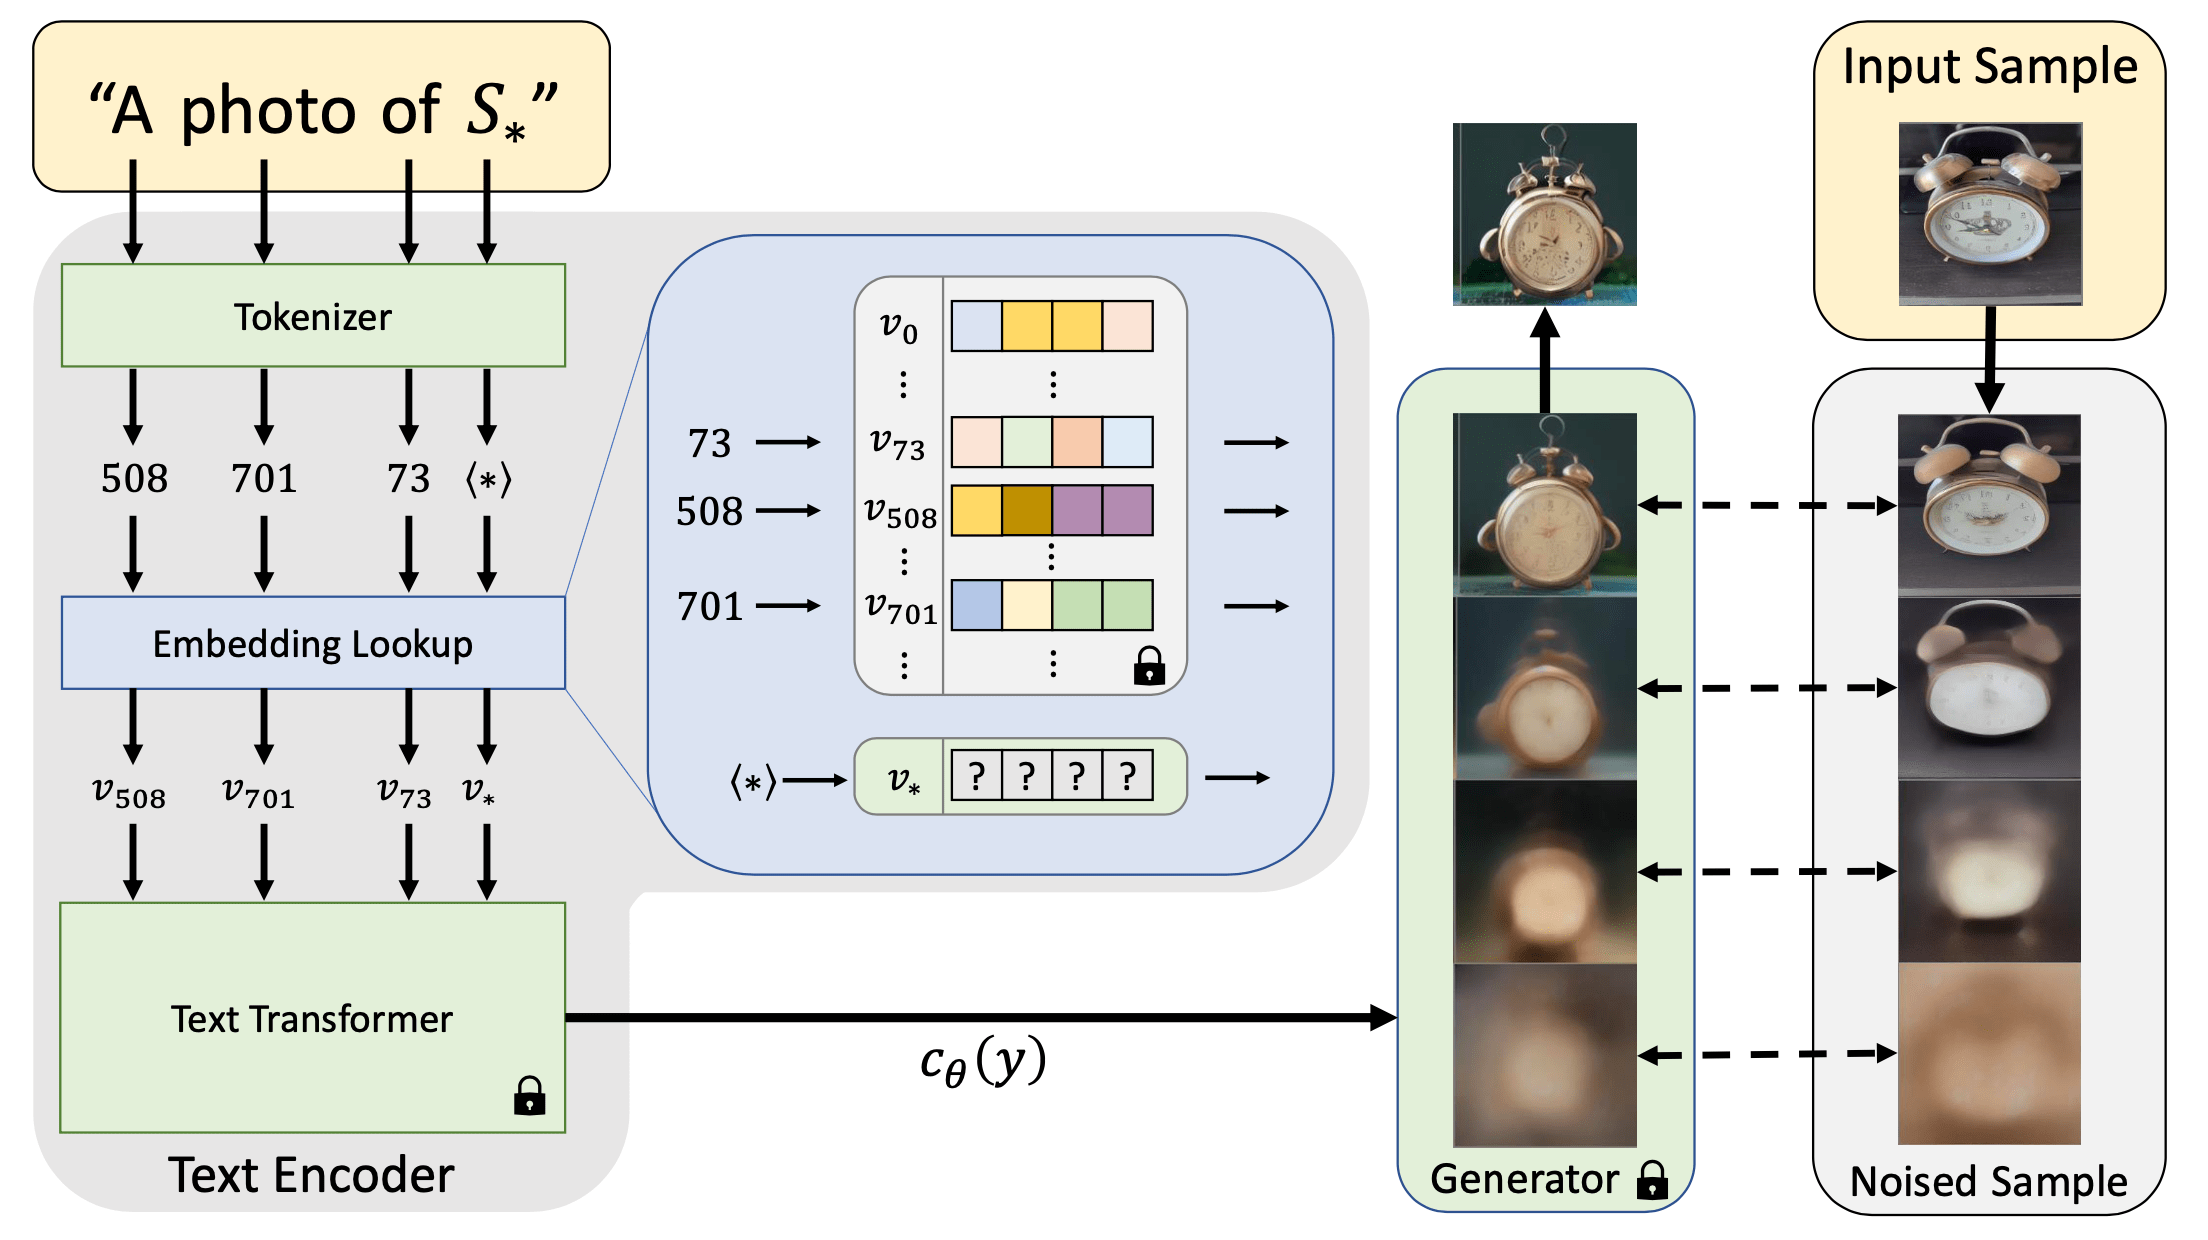
\includegraphics[width=0.9\textwidth]{Pictures/textualI.png} 
    \caption{\textbf{Outline of the text-embedding and inversion process} \cite{gal2022image}. The input containing the placeholder \textit{S∗} is converted to tokens and, subsequently, to embedding vectors. Finally, the embedding vectors condition the generation through the conditioning code $c_{\theta }(y)$.}
    \label{fig:textualI}
\end{figure}

\subsection{Dreambooth}

The Dreambooth approach consists of taking a few images of the subject to be generated together with the name of the corresponding class and returning the fine-tuned model with a unique identifier referring to the subject. This approach presents two significant problems related to overfitting and forgetting how to generate images of other subjects of the same class. To solve this, the authors propose using a \textit{class-specific prior preservation loss}. This loss function is based on supervising the model with its own generated images.

Furthermore, the fine-tuning process involves two steps. Initially, it is performed on the section dedicated to the low-resolution model, where the loss function is applied to avoid language drift and overfitting. Subsequently, fine-tuning is performed on the super-resolution section with examples in high and low resolution to maintain the subject's small details. An overview of the process can is shown in figure \ref{fig:dreamboothS}.

\begin{figure}
    \centering
    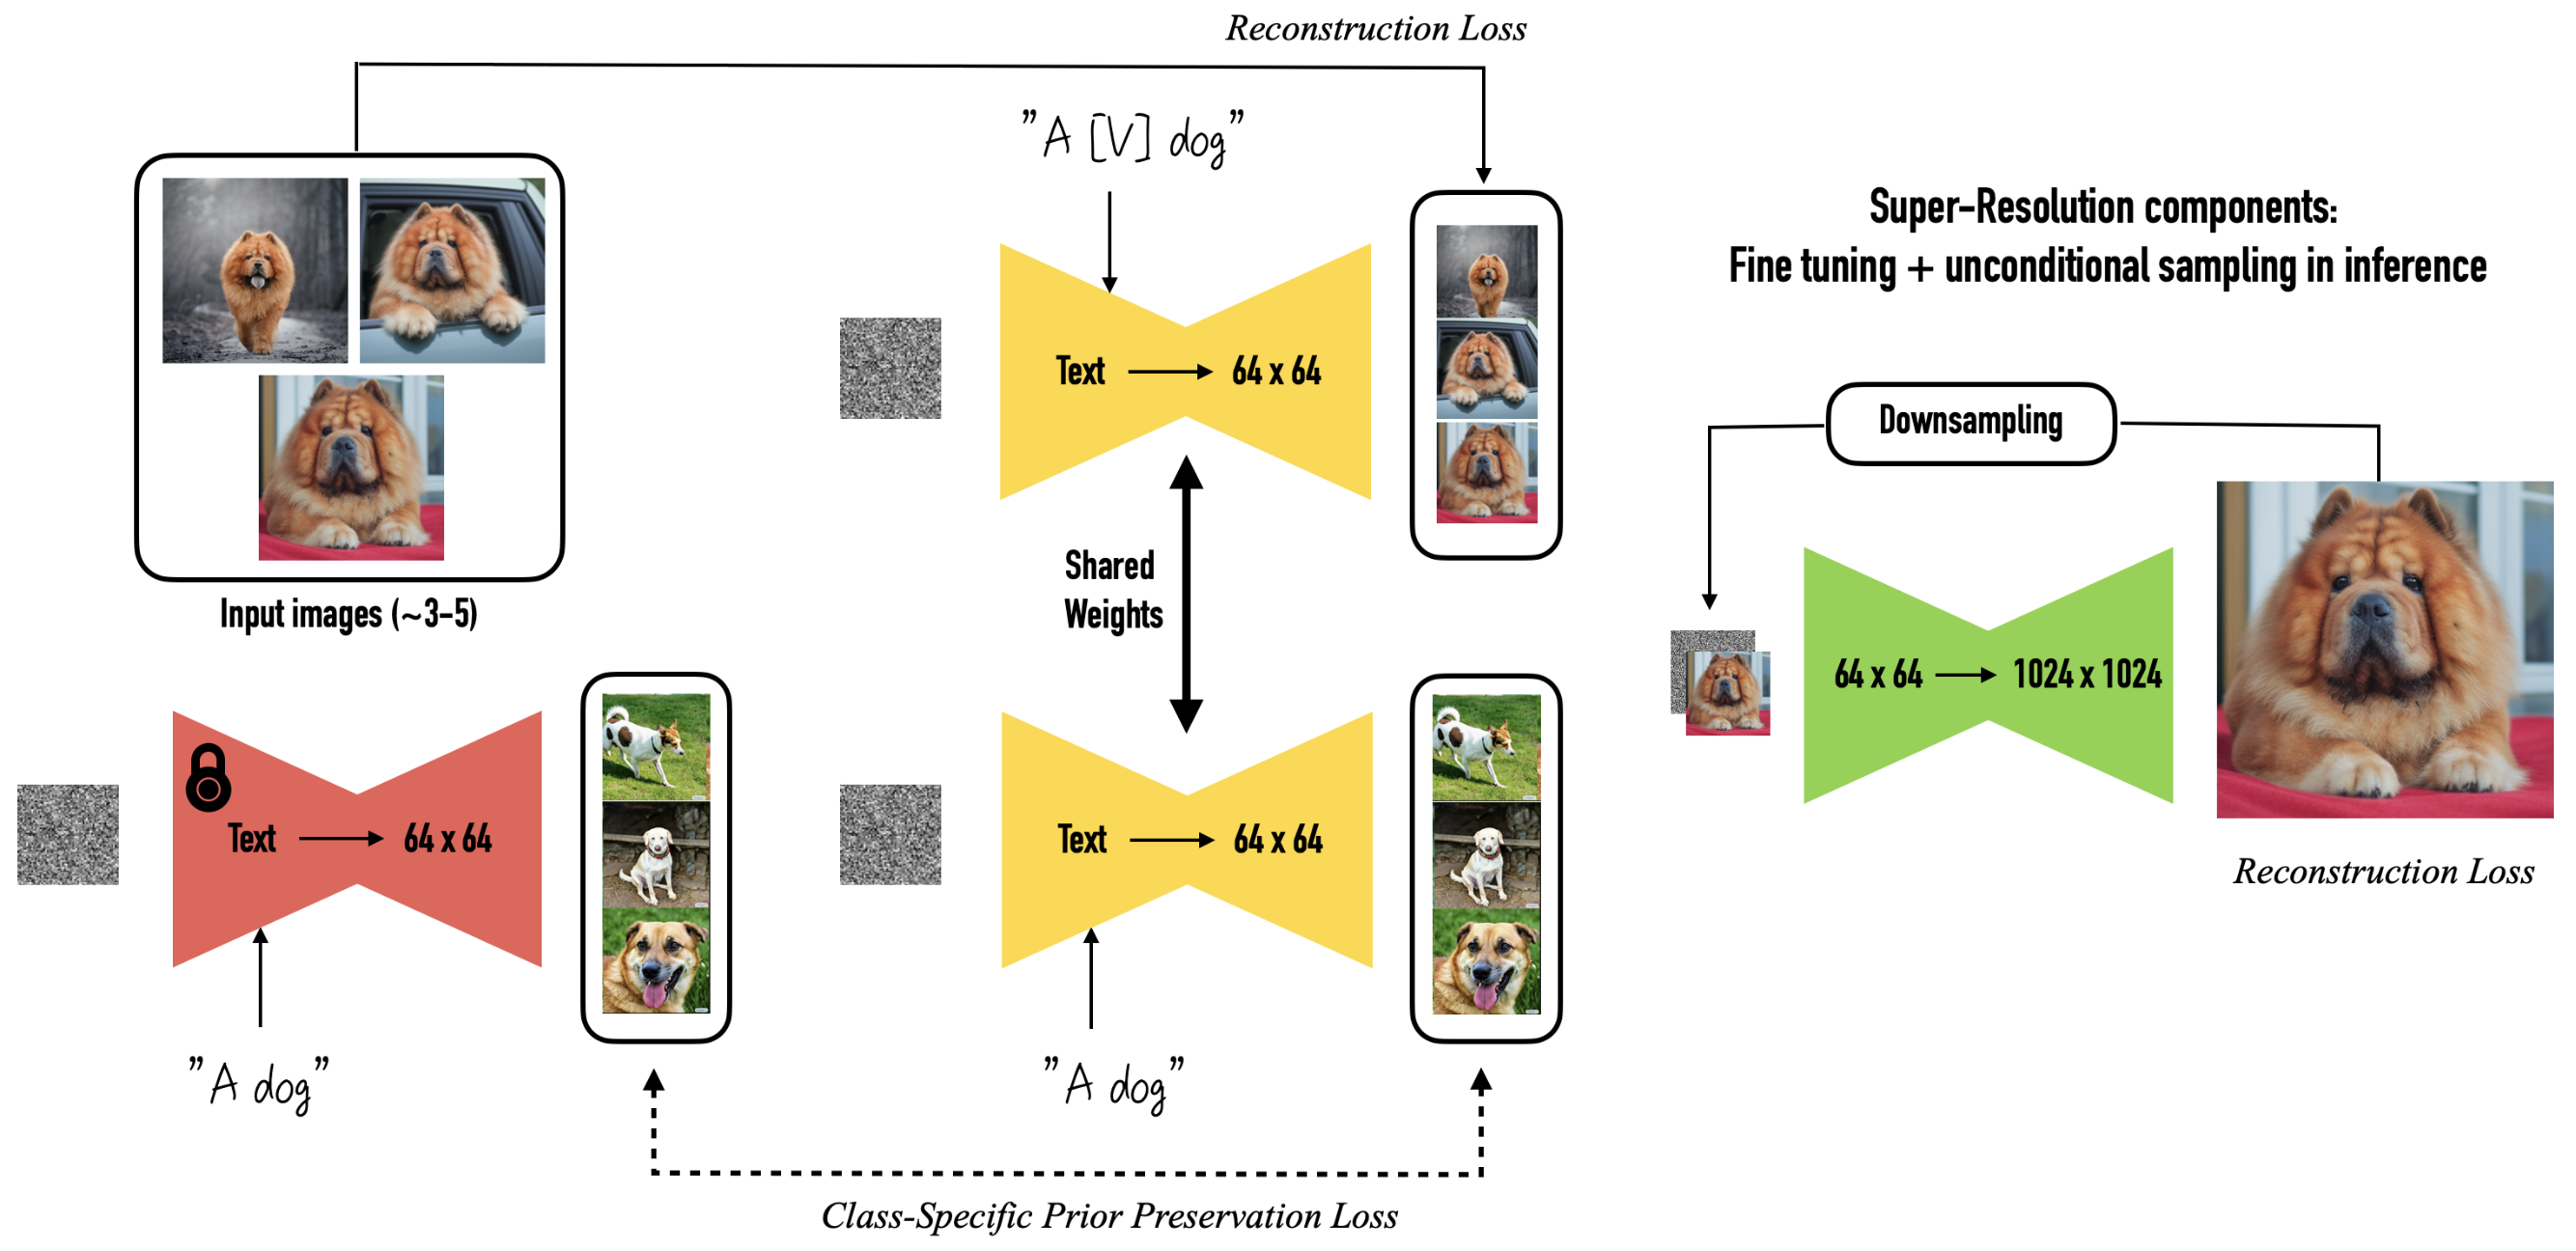
\includegraphics[width=0.9\textwidth]{Pictures/dreamboothS.png} 
    \caption{\textbf{Fine-tuning process for Dreambooth} \cite{ruiz2023dreambooth}. Two main steps are distinguished. First, fine-tuning is performed on the low-resolution section, where the class-specific prior preservation loss is applied. On the other hand, fine-tuning the high-resolution section with pairs of high and low-resolution images makes it possible to keep the subject detail.}
    \label{fig:dreamboothS}
\end{figure}

\section{Conditional control}

Text-based image creation models offer exceptional flexibility due to the highly adaptable nature of the text input they receive. In addition, areas of study such as \textit{subject-driven generation} have further extended the possibilities of these models. However, there are still significant shortcomings in the control of the generated image, for instance, in the control of the anatomy of people or the arrangement of objects in a scene. These weaknesses are why ControlNet \cite{zhang2023adding} was created with the aim of controlling large text-to-image models to learn specific input conditions. 

ControlNet is a neural network architecture. This structure works by creating two copies of the weights of a text-to-image model. One copy will be ``\textit{trainable}" and the other ``\textit{locked}". The first one is trained to learn conditional control for specific tasks. In contrast, the second remains intact to maintain the network's capabilities. These two copies are then connected through a type of convolution layer called ``\textit{zero convolution}". This layer is a 1x1 convolution layer with its weights initialised to zero in order not to introduce noise in the deep features and thus allow the training to be fast. 

Hence, the proposed architecture modifies the input conditions of the different blocks of layers comprising a neural network. Figure \ref{fig:controlNetD} shows how the structure of the neural network blocks is changed to condition the neural network. Thus, with the addition of the deep features of the network with the desired condition, the ``trainable" copy can be trained in order to subsequently be added with the deep features derived from the ``locked" copy. 

\begin{figure}
    \centering
    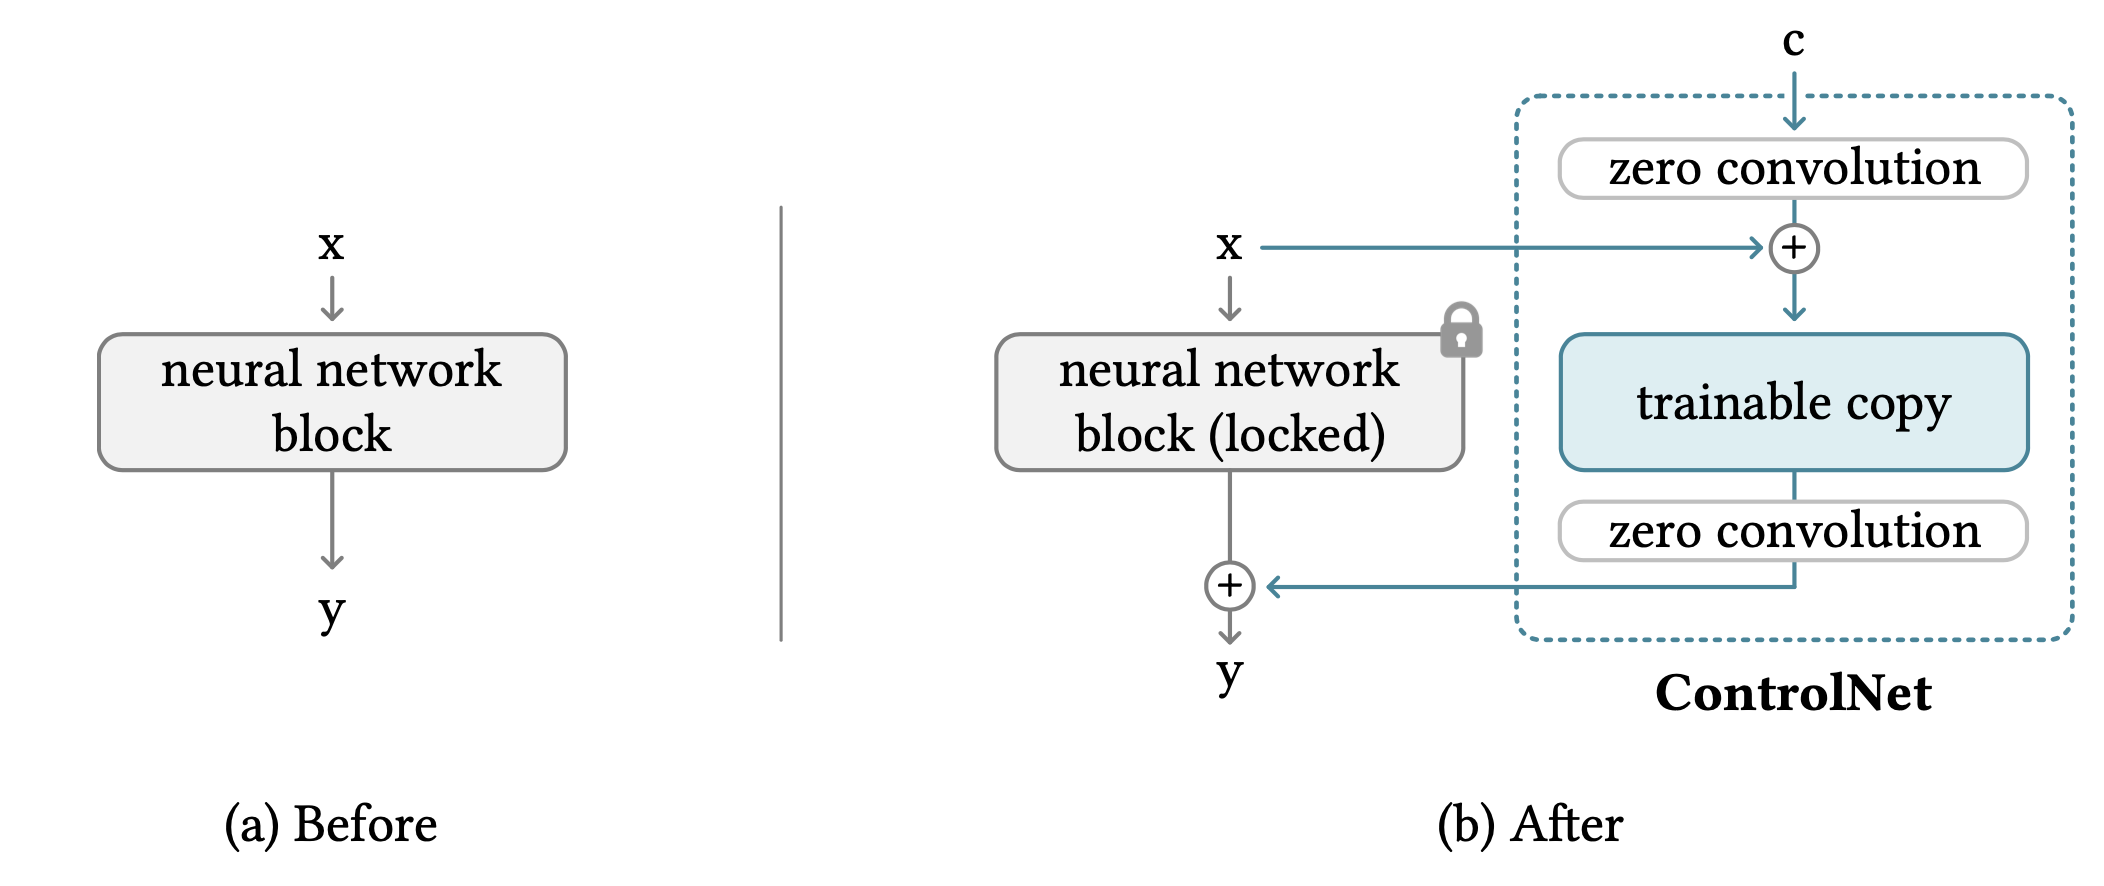
\includegraphics[width=1\textwidth]{Pictures/controlNetD.png} 
    \caption{\textbf{ControlNet architecture} \cite{zhang2023adding}. The deep feature \textit{x} gets added with the condition \textit{c} to get passed to the \textit{trainable} copy. Meanwhile, the output of the \textit{locked} copy after getting \textit{x} as input is added to the output of the trainable copy to produce the deep feature \textit{y} already conditioned.}
    \label{fig:controlNetD}
\end{figure}

The ControlNet authors provide a list of trained networks with different conditioning modes. Some of the most useful are Canny edges, segmentation maps, depth maps or scribbles. Image \ref{fig:controlNetE} shows some of these conditioning examples.

\begin{figure}
    \centering
    \includegraphics[width=1\textwidth]{Pictures/controlNetE.png} 
    \caption{\textbf{Control of Stable Diffusion with ControlNet trained on Canny edge, Openpose, Hough lines and Openpifpaf pose} \cite{zhang2023adding}.}
    \label{fig:controlNetE}
\end{figure}

\section{Data augmentation}

Data augmentation is a technique used in the field of machine learning to improve the performance of models. The idea behind this concept is to increase the diversity of the training data in order to teach the model to deal more accurately with real data. In other words, the aim is to improve the generalisability of machine learning models. However, despite the great potential of the idea, most research has focused on creating better and better architectures instead of improving the already existing data augmentation techniques \cite{cubuk2018autoaugment}.

Generally speaking, most data augmentation techniques applied to real problems are designed \textit{ad-hoc}. The reason for this fact is that not all available transformations make sense in all cases. For example, the horizontal flipping transformation does not make sense in the MNIST digit recognition task. Consequently, the creation of augmentations requires prior experience of machine learning experts and slows down and makes the creation of computer vision models more expensive. So much so that in 2018 OpenAI considered the automatic search for augmentations an unsolved problem \cite{requestsresearch}.

In response to this problem, Google Brain researchers formulated \textit{AutoAugment} \cite{cubuk2018autoaugment} in 2019. This data augmentation technique automatically searches for the best combinations of transformations to create a policy that obtains good results without needing careful, ad-hoc design. To achieve this, they formulate the task as a discrete search problem. The search space consists of a policy with 5 sub-policies, where each sub-policy consists of 2 transformations that are applied to the images. Their results show state-of-the-art accuracy on ImageNet and CIFAR-10 and demonstrate that the learned policies can also be transferred to other datasets with state-of-the-art results.

Despite the promising results obtained by \textit{automated augmentation policies} \cite{cubuk2018autoaugment}, their computational cost makes their massive use in training deep learning models impossible. Their higher computational cost is because they require an additional search phase. Therefore, although the improvement of the models' results is palpable, the dual learning process in which the network is trained simultaneously as a search is performed in the augmentations space implies a computational complexity that is not feasible in many tasks. In the original \textit{AutoAugment} publication, they try to provide a solution by performing the search task in a minor task than the original one. They then transfer the result to the original larger task. However, Google Brain, in the publication \textit{RandAugment: Practical automated data augmentation with a reduced search space} \cite{cubuk2020randaugment}, finds evidence that contradicts the approach. Thus, they propose a new automated augmentation technique that solves the problems raised by eliminating the search task. Consequently, they propose to reduce the search space so much that it allows them to find the best combination using only grid search on the 2 hyperparameters they propose.

On the other hand, the scientific community has also explored techniques to create new training data. Thus, not all efforts have been based on transforming the data itself. Instead, some have been on creating new data automatically. One of the most exciting directions taken in recent years is \textit{Copy-Paste augmentation} for segmentation tasks. The idea is to take objects from some images and place them in the backgrounds of other images. In this way, new training images are created for free. Moreover, this idea presents many combinations and allows to explore many ways of doing it. One of the most successful attempts is detailed in \textit{Simple Copy-Paste is a Strong Data Augmentation Method for Instance Segmentation} \cite{ghiasi2021simple}. In this publication, researchers demonstrate that a simple strategy in which random objects are taken and pasted into random locations produces results that improve the baselines of multiple problems. Figure \ref{fig:copy-paste} shows the result of applying this technique to two images.

\begin{figure}
    \centering
    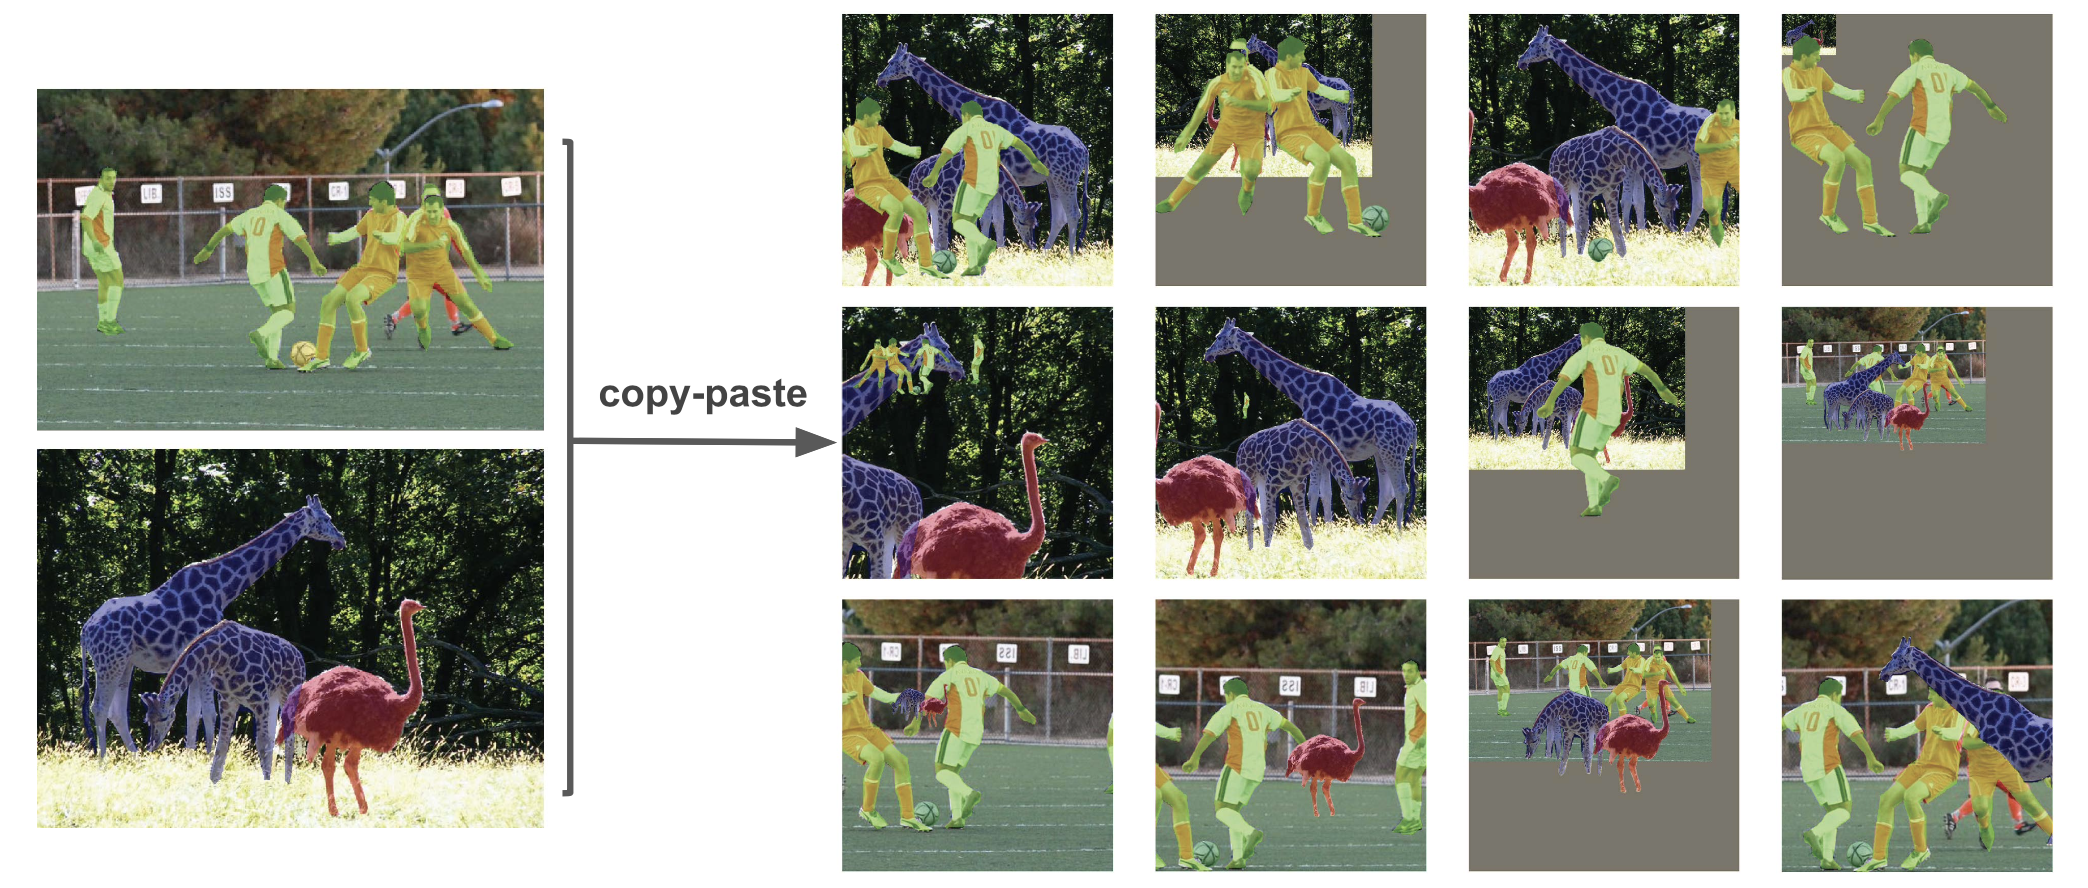
\includegraphics[width=1\textwidth]{Pictures/copy-paste.png} 
    \caption{\textbf{Simple Copy-Paste augmentation} \cite{ghiasi2021simple}. This technique generates new training images by copying objects from one image into the background of another. Moreover, standard scale jittering (SSJ) and large scale jittering (LSJ) are used to randomly resize and crop images.}
    \label{fig:copy-paste}
\end{figure}

The next logical step in creating new training data is to take text-to-image models. Thus, the \textit{generative data augmentation} trend has come with the explosion in the capabilities of such models seen in recent years \cite{rombach2022high, dhariwal2021diffusion}. This trend proposes using sufficiently advanced image generation models to create entirely new images in the training dataset. Thus, the approach consists of synthetically increasing the diversity of the data. In this line, very recent works (April 2023), such as \textit{Synthetic Data from Diffusion Models Improves ImageNet Classification} \cite{azizi2023synthetic}, are unmistakable with their results. They show that augmenting training data with images generated by text-to-image models creates models that significantly improve past baselines. Furthermore, other works show that it is possible to train full classification models with just synthetic images and obtain competitive results \cite{sariyildiz2023fake}. In line with these two publications, \textbf{the present work aims to test the effectiveness of subject-driven generation techniques to increase the performance of classification and segmentation models}.